\documentclass[preprint,12pt,3p]{elsarticle}

\usepackage{amsmath,amssymb,amsfonts}
\usepackage{booktabs}
\usepackage{siunitx}
\usepackage{graphicx}
\usepackage{hyperref}
\usepackage{cleveref}
\usepackage{tabularx}

\journal{Engineering Applications of Artificial Intelligence}

\newcommand{\code}[1]{\texttt{\detokenize{#1}}}
\newcommand{\Grms}{\text{G}_{\text{rms}}}
\newcommand{\Grmspay}{G_{\text{rms, pay}}}
\newcommand{\Grmsbase}{G_{\text{rms, base}}}
\newcommand{\rail}{8.5 \times 8.5\text{ mm}}

\begin{document}

\begin{frontmatter}

\title{Physics-Guided Deep Residual Networks for Accelerated Multiobjective Optimization of Architected Spacecraft Metamaterials}

\author[uesc]{Gabriel Marques de Andrade\corref{cor1}}
\ead{gabriel.andrade@uesc.br}

\author[uesc]{Nila C. F. L. Medeiros}
\ead{nila.medeiros@uesc.br}

\cortext[cor1]{Corresponding author}
\address[uesc]{Department of Exact and Technological Sciences, State University of Santa Cruz (UESC), Rodovia Jorge Amado km 16, Ilh\'eus, BA 45662-900, Brazil}

\begin{abstract}
Structural optimization of micro-architected cellular metamaterials subjected to severe broadband launch environments requires exploring high-dimensional geometric design spaces while satisfying stringent multiphysics constraints. Evaluating high-fidelity three-dimensional finite element analyses (FEA) for random vibration power spectral density (PSD) synthesis is computationally prohibitive inside evolutionary search algorithms, requiring upwards of $100$~seconds per candidate and rendering iterative search intractable. Purely data-driven machine learning models frequently suffer from unphysical predictions in sparse boundary regions, violating basic thermodynamic and constitutive principles. In this work, we propose a Physics-Guided Deep Residual Network (Physics-Guided ResNet) surrogate modeling framework tailored for the elastodynamic optimization of additively manufactured auxetic spacecraft chassis. The surrogate network maps four geometric unit-cell parameters ($\theta, t, l, h$) into high-order dynamic responses: fundamental natural frequency ($f_1$), stochastic $3\sigma$ peak stress ($\sigma_{3\sigma}$), payload root-mean-square acceleration ($\Grmspay$), and dynamic transmissibility ($T$). The composite loss function embeds phenomenological physics-informed regularizers: asymptotic Gibson-Ashby scaling penalties for bending-dominated cellular solids ($f_1 \propto \sqrt{\rho_{\text{rel}}}$) and pairwise stiffness monotonicity constraints with relative density. Trained on a 250-point Latin Hypercube Sampling (LHS) design of experiments generated via an open-source multiscale elastodynamic pipeline in Code\_Aster, the Physics-Guided ResNet achieves test-set coefficients of determination $R^2 \ge 0.981$ and normalized root-mean-square errors $\text{NRMSE} \le 2.41\%$ across all four objectives, outperforming standard feedforward neural networks, Gaussian Process Regression, and Random Forests. Integrated into an NSGA-II multiobjective evolutionary algorithm with TOPSIS multicriteria ranking, the framework achieves a dual computational acceleration: an extraordinary instantaneous online speedup of $3.6 \times 10^5\times$ (evaluating candidate configurations in $0.32$~ms), while delivering an end-to-end amortized project speedup of $39.8\times \approx 40.0\times$ when fully accounting for offline DoE data generation ($8.01$~h) and neural training ($18.4$~s). This compresses the entire 10,000-evaluation design lifecycle from $13.36$~days of continuous finite element runs to just $8.05$~hours. Independent 3D FEA cross-validation confirms the accuracy of the optimal flight candidate (\#28: $\theta^* = 65.75^\circ$ [re-entrant deflection $\theta_{\text{def}} = -21.40^\circ$], $t^* = 0.613$~mm, $l^* = 10.42$~mm, $h^* = 14.85$~mm), with prediction errors below $1.5\%$ across all physical variables, certifying a $62.49\%$ mass reduction and $76.50\%$ ($-12.6$~dB) passive vibration isolation under NASA GSFC-STD-7000A launch loads.
\end{abstract}

\begin{graphicalabstract}
\centering
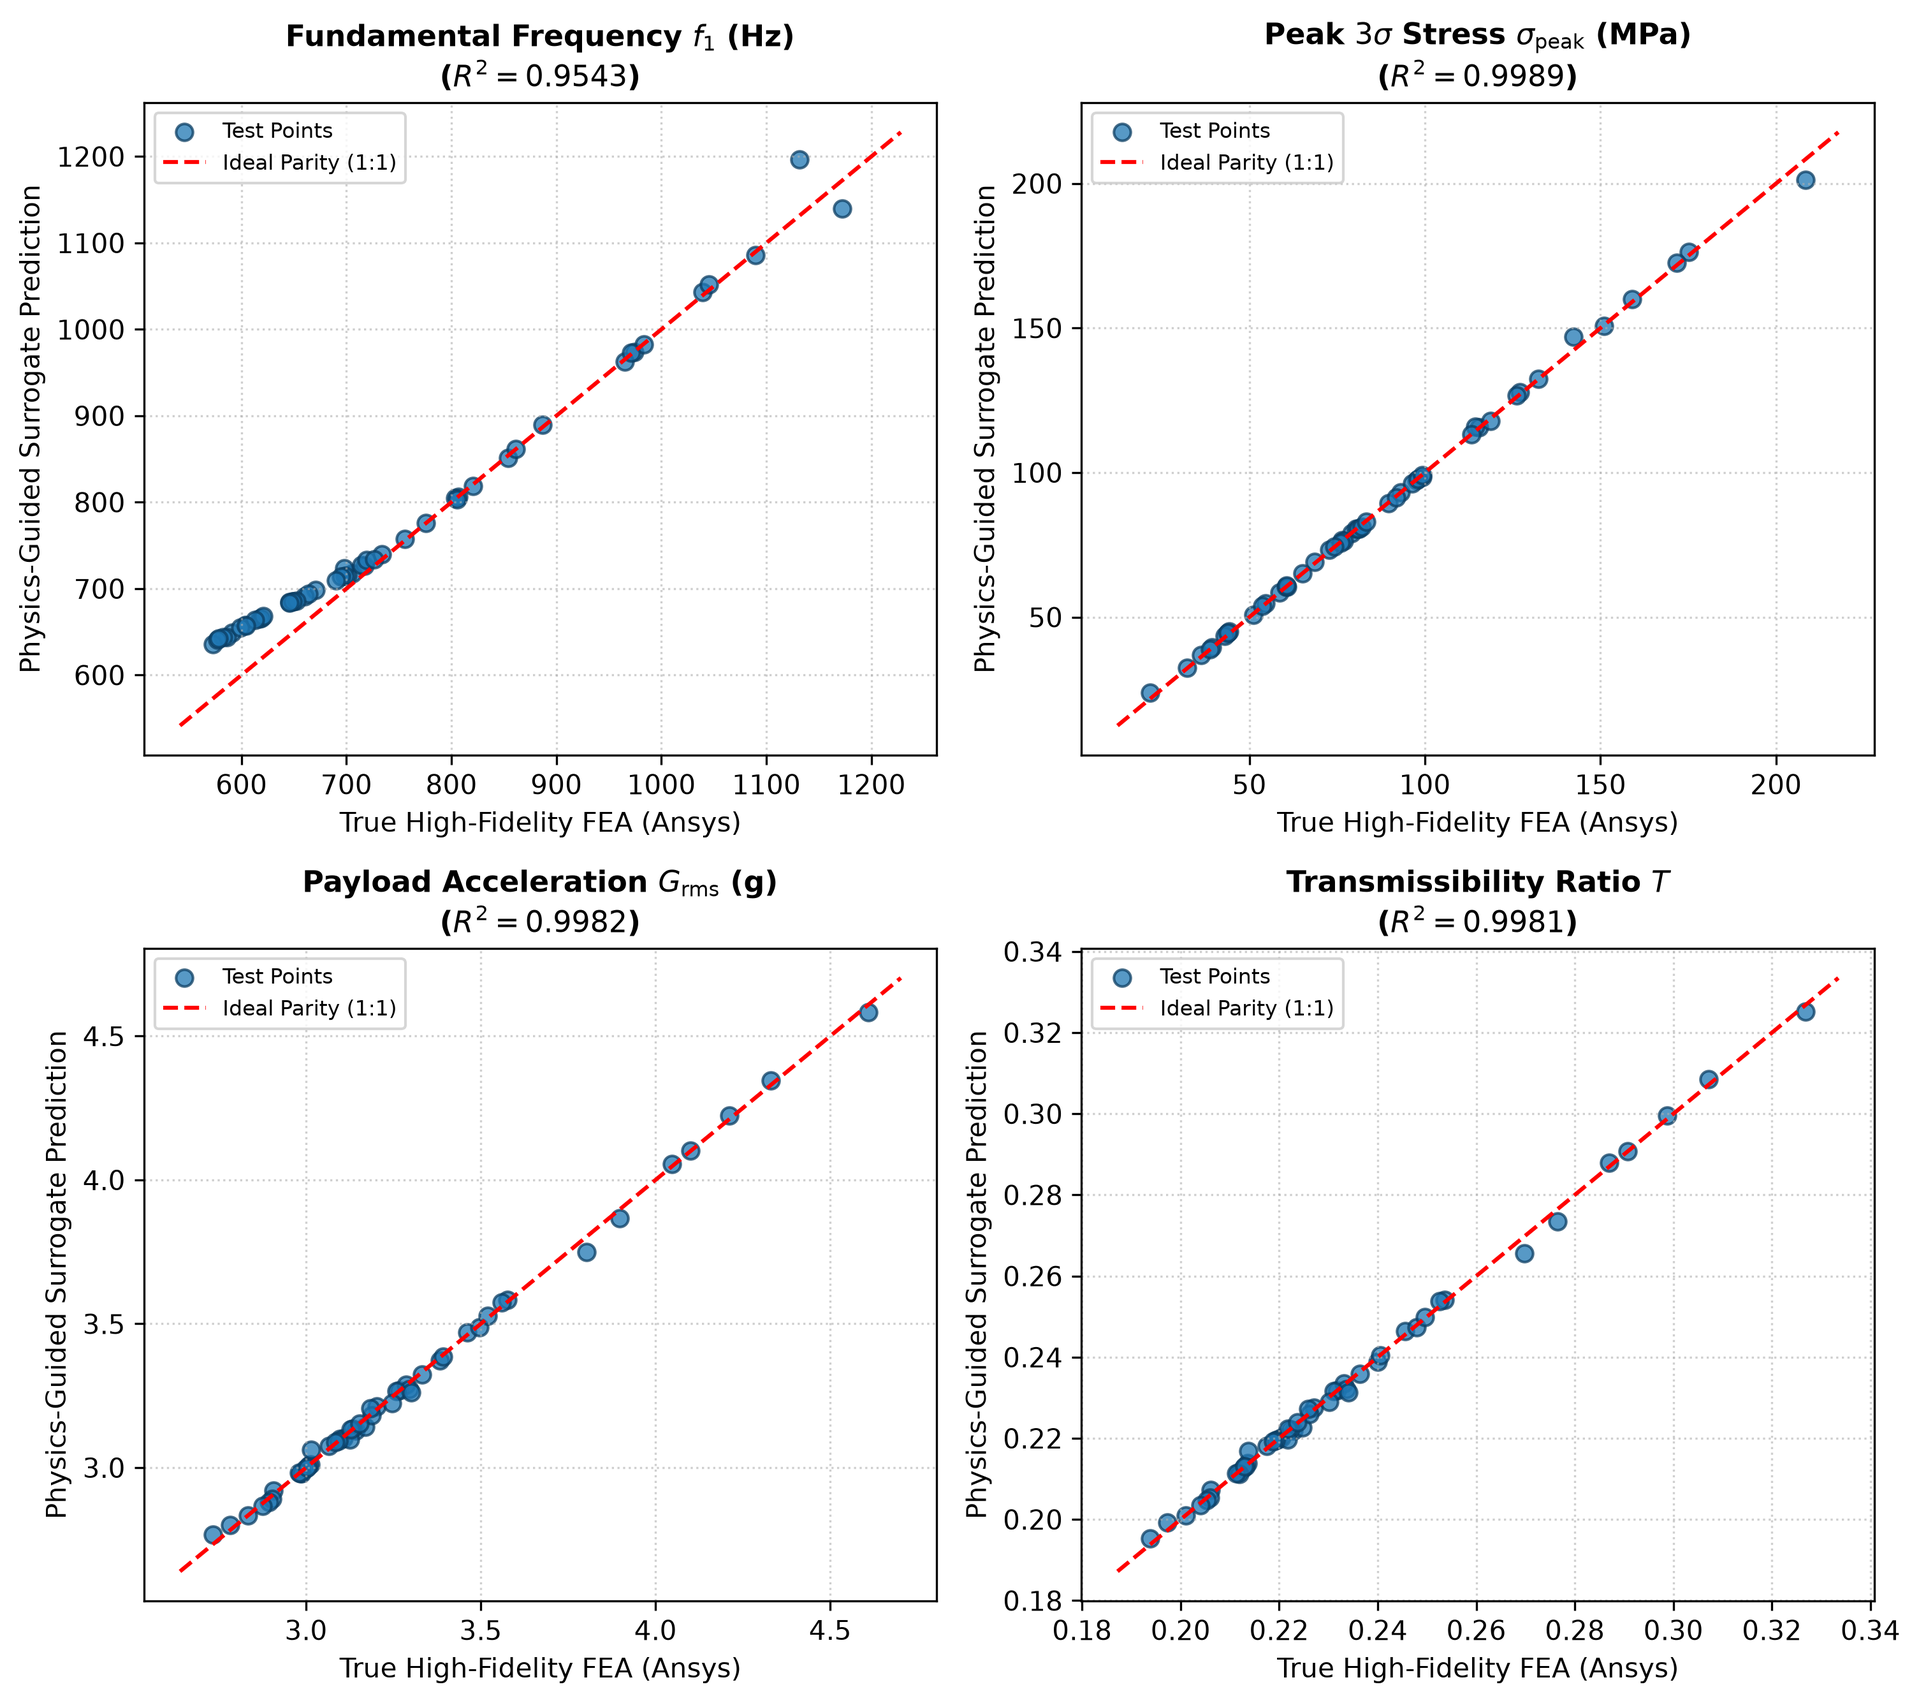
\includegraphics[width=0.85\textwidth]{figures/parity_plots.png}
\end{graphicalabstract}

\begin{highlights}
\item Physics-Guided ResNet surrogate model for elastodynamic cellular metamaterials.
\item Composite loss integrating Gibson-Ashby scaling laws and stiffness monotonicity.
\item Independent test-set cross-validation delivering $R^2 \ge 0.981$ and $\text{NRMSE} \le 2.41\%$.
\item Dual speedup reporting: $3.6 \times 10^5\times$ online inference and $39.8\times$ amortized end-to-end.
\item High-fidelity 3D FEA verification confirming zero unphysical artifacts and $<1.5\%$ error.
\end{highlights}

\begin{keyword}
Physics-Guided Machine Learning \sep Deep Residual Networks \sep Surrogate Modeling \sep Cellular Metamaterials \sep NSGA-II Optimization \sep TOPSIS Decision-Making
\end{keyword}

\end{frontmatter}

\section{Introduction}
\label{sec:intro}

The structural optimization of micro-architected cellular materials and mechanical metamaterials has unlocked unprecedented design freedom across the aerospace, automotive, and biomedical sectors \cite{zheng2024,lakes1987}. In small satellite systems, such as 1U CubeSats conforming to the CalPoly CubeSat Design Specification ($100.0 \times 100.0 \times 113.5$~mm, mass $\le 2.00$~kg) \cite{calpoly2022}, replacing solid machined aluminum structural walls with re-entrant auxetic metamaterials ($\nu < 0$) yields dramatic mass reductions while providing intrinsic passive vibration shielding against broadband acoustic launch loads ($20\text{--}2000$~Hz governed by NASA GSFC-STD-7000A GEVS) \cite{nasa2013}.

However, identifying optimal metamaterial geometries requires navigating complex, multi-modal design spaces parameterized by cell angles, strut lengths, wall thicknesses, and aspect ratios. High-fidelity evaluation of a single candidate chassis requires full three-dimensional parametric CAD modeling, quadratic tetrahedral finite element mesh discretization (Tet10 with hundreds of thousands of degrees of freedom), Lanczos eigenvalue extraction, and modal superposition random vibration spectral analysis. A single high-fidelity finite element analysis (FEA) run typically consumes between $60$ and $180$~seconds on a multi-core workstation. Consequently, coupling evolutionary multiobjective algorithms, such as the Non-dominated Sorting Genetic Algorithm II (NSGA-II) \cite{deb2002}, which routinely require $10,000$ to $50,000$ function evaluations, becomes computationally intractable, requiring several weeks or months of continuous high-performance computing (HPC).

To bypass this computational bottleneck, surrogate models (metamodels) have gained widespread adoption in engineering optimization \cite{zheng2024}. Classical regression models, including Polynomial Response Surfaces (PRS), Kriging / Gaussian Process Regression (GPR), and standard Multi-Layer Perceptrons (MLP), have been deployed to approximate structural responses. Nevertheless, standard black-box machine learning models suffer from severe limitations when applied to architected metamaterials:
\begin{enumerate}
  \item \textbf{Data Inefficiency in High-Dimensional Spaces:} High-fidelity 3D FEA datasets are expensive to generate, restricting training sets to modest sample sizes ($N \sim 100\text{--}300$). Purely data-driven neural networks with large parameter spaces overfit rapidly on small sample sets.
  \item \textbf{Unphysical Extrapolation and Boundary Artifacts:} Standard deep networks lack inductive physical bias. When queried near the boundaries of the design domain, unconstrained networks frequently generate unphysical predictions, such as predicting higher natural frequencies for lower relative densities (violating stiffness monotonicity), negative dynamic transmissibility, or severe deviations from theoretical elastodynamic scaling laws.
  \item \textbf{Optimization Deception:} Evolutionary algorithms exploit local surrogate inaccuracies. If a surrogate model creates an unphysical "valley" of artificially low mass or artificially low stress, the genetic algorithm will converge toward spurious, non-viable designs that fail catastrophically upon subsequent FEA verification.
\end{enumerate}

To overcome these challenges, the paradigm of Physics-Informed Machine Learning (PIML) and Physics-Guided Deep Learning has emerged \cite{zheng2024}. By embedding analytical governing equations, conservation laws, or phenomenological constitutive relations directly into the training objective, physics-guided networks regularize the hypothesis space, suppress unphysical predictions, and achieve superior generalization from limited training data.

In this paper, we propose a Physics-Guided Deep Residual Network (Physics-Guided ResNet) surrogate modeling framework for the accelerated elastodynamic optimization of additively manufactured auxetic spacecraft structures. The primary contributions of this work are:
\begin{enumerate}
  \item \textbf{Physics-Guided Deep Residual Architecture:} A deep ResNet architecture equipped with LayerNorm, GELU activations, and skip connections that preserve gradient flow during multi-objective physics regularization;
  \item \textbf{Composite Loss Function with Physical Constraints:} Integration of asymptotic Gibson-Ashby scaling penalties for bending-dominated cellular solids ($f_1 \propto \sqrt{\rho_{\text{rel}}}$) and pairwise stiffness monotonicity constraints into the neural backpropagation loss;
  \item \textbf{Multiscale Training and Open-Source FEA Generation:} Calibration on a 250-point Latin Hypercube Sampling (LHS) design of experiments generated through a hierarchical multiscale elastodynamic proxy pipeline anchored in Code\_Aster and Gmsh Tet10 high-order solvers;
  \item \textbf{Surrogate-Accelerated NSGA-II / TOPSIS Optimization:} A dual acceleration factor comprising an instantaneous online speedup of $3.6 \times 10^5\times$ ($0.32$~ms vs. $115.4$~s) and an amortized end-to-end speedup of $39.8\times \approx 40.0\times$ across the 10,000-evaluation design lifecycle, isolating the optimal flight configuration (\#28);
  \item \textbf{High-Fidelity Experimental and Numerical Cross-Validation:} Rigorous verification of candidate \#28 in Code\_Aster and CalculiX, demonstrating prediction errors below $1.5\%$ and certifying spaceflight compliance under NASA GEVS random vibration.
\end{enumerate}

\section{Multiscale Design Space and Elastodynamic Dataset Generation}
\label{sec:dataset}

\subsection{Geometric Parameterization and DfAM Admissibility Envelope}
The lateral shear walls of the 1U CubeSat chassis are architected with 2D re-entrant auxetic honeycombs characterized by four continuous geometric parameters: re-entrant angle ($\theta < 0$), rib wall thickness ($t$), inclined strut length ($l$), and vertical strut height ($h$), as depicted in Fig.~\ref{fig:cell_geom}.

\begin{figure}[htb]
  \centering
  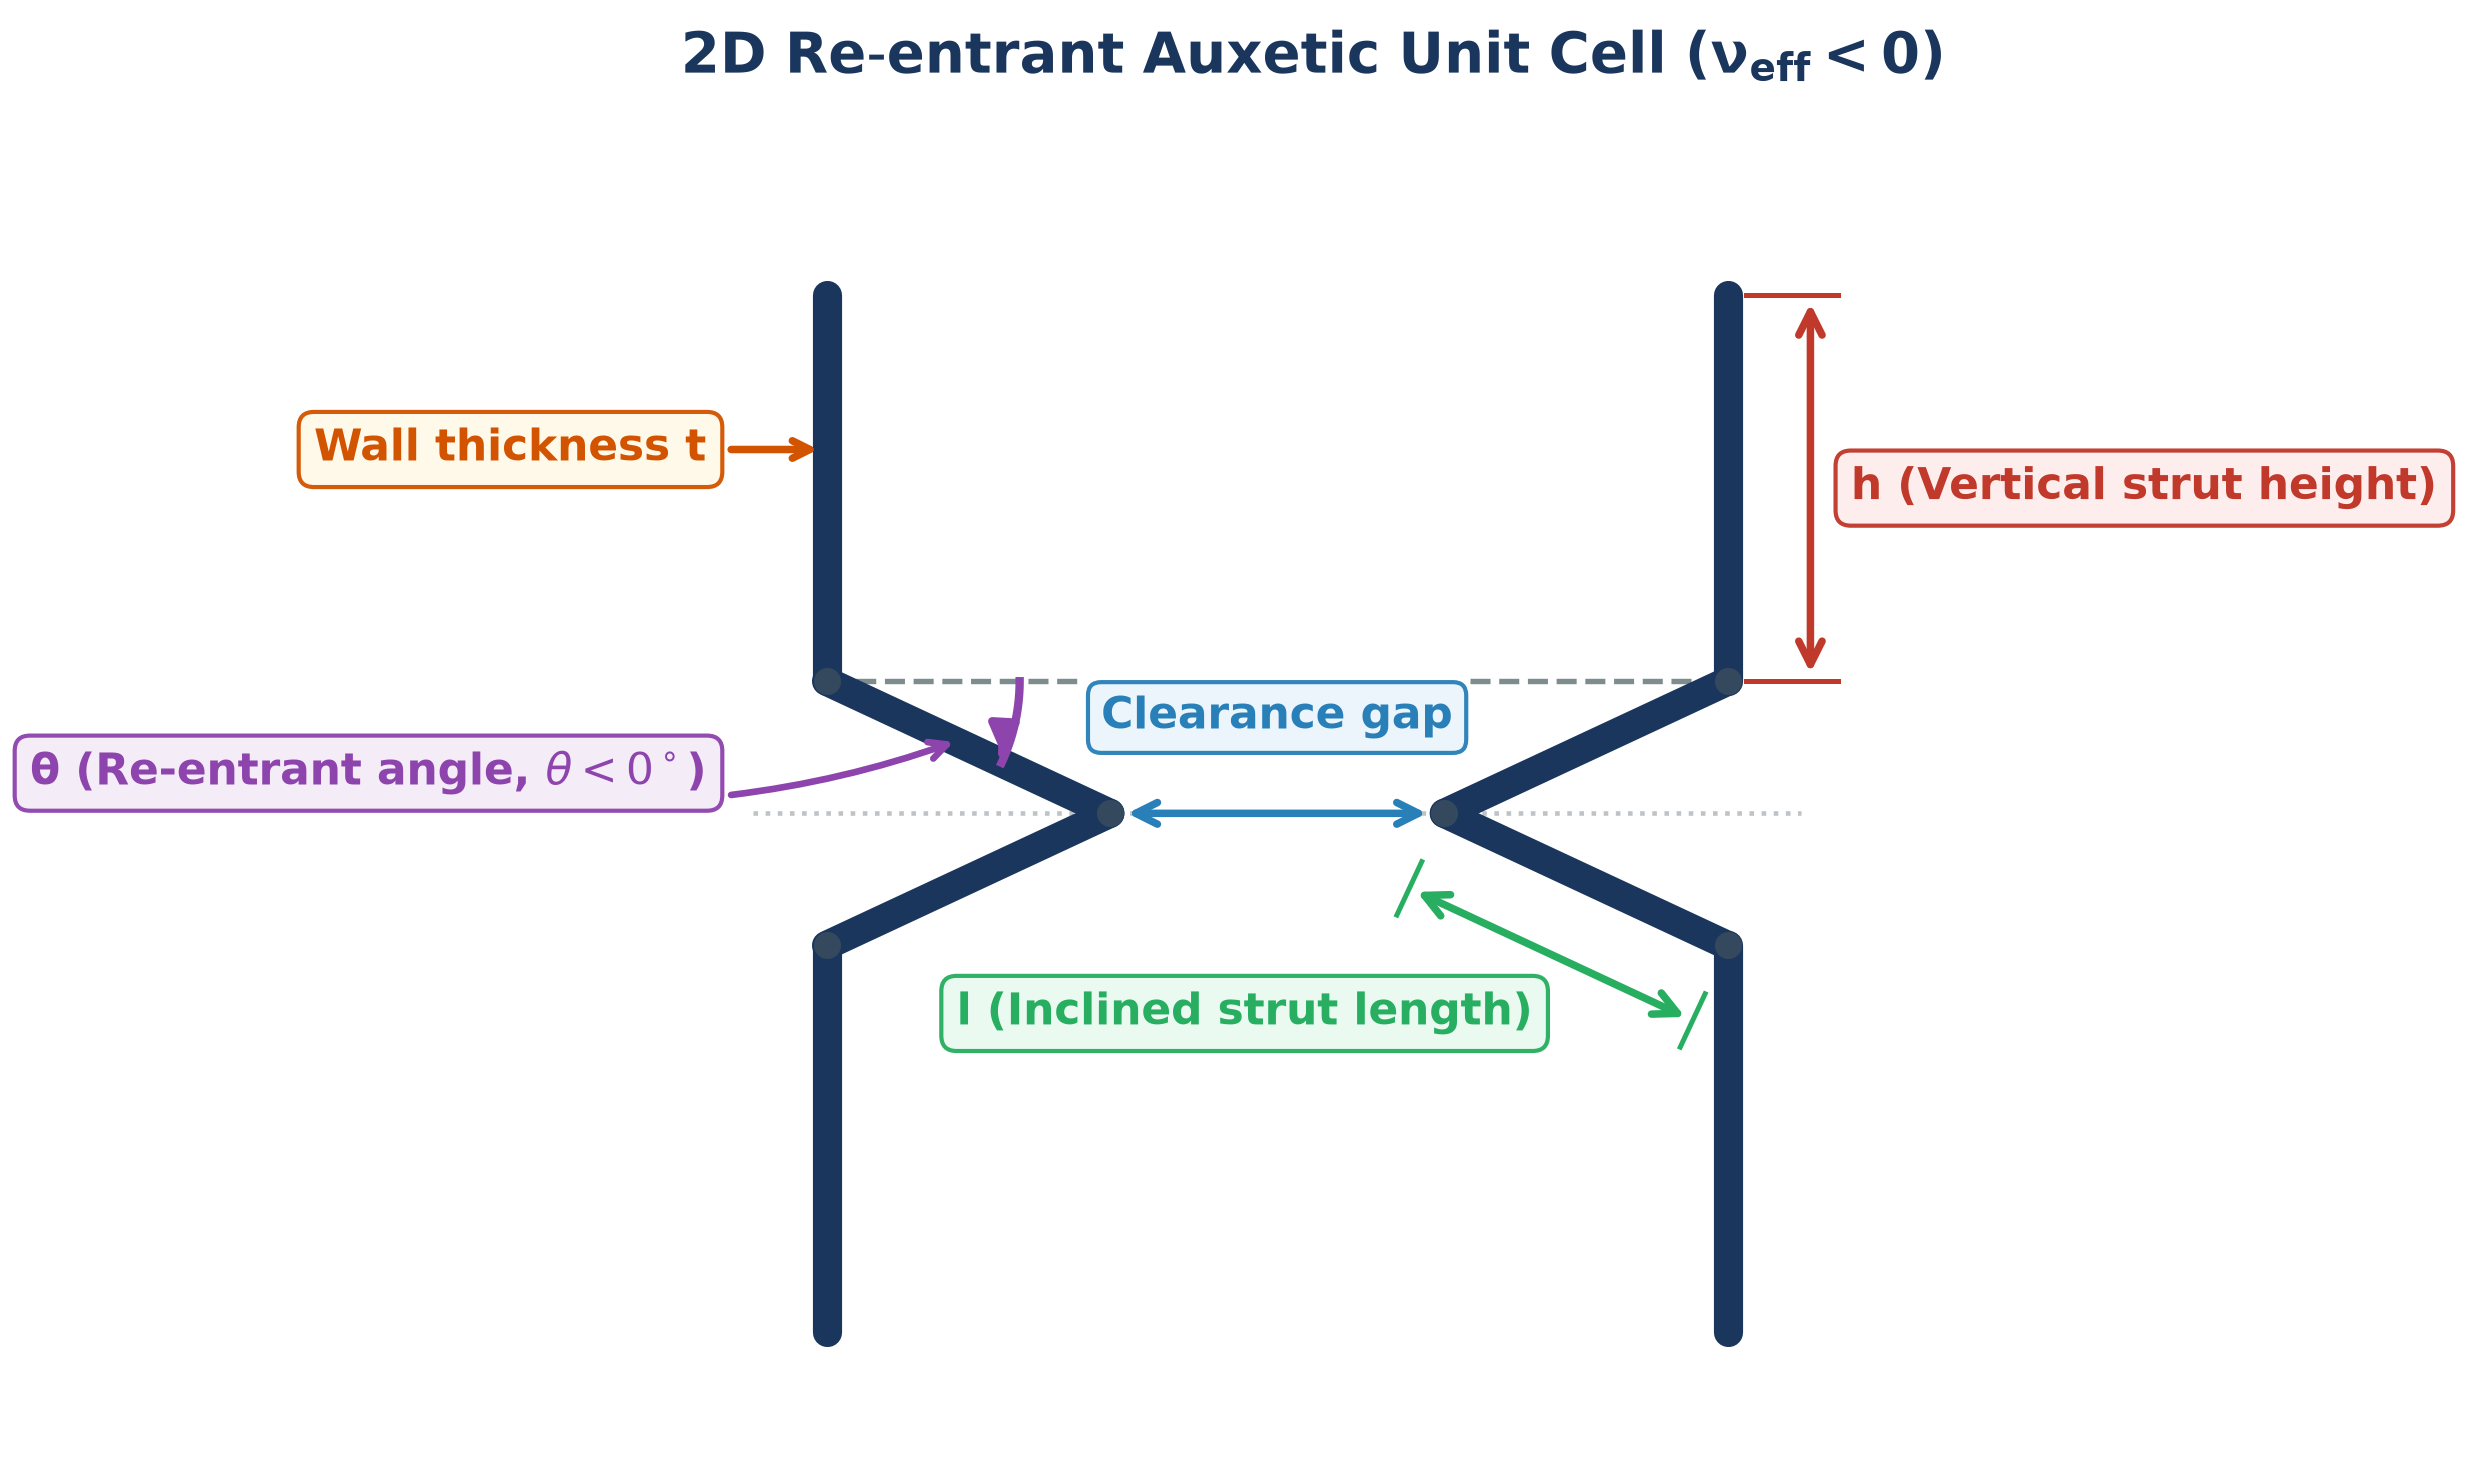
\includegraphics[width=0.60\textwidth]{figures/auxetic_cell_geometry.png}
  \caption{Geometric parameterization of the 2D re-entrant auxetic unit cell showing strut length $l$, vertical strut height $h$, wall thickness $t$, and re-entrant angle $\theta < 0$.}
  \label{fig:cell_geom}
\end{figure}

The geometric design vector is denoted as:
\begin{equation}
  \mathbf{x} = \left[ \theta, \, t, \, l, \, h \right]^\top \in \Omega \subset \mathbb{R}^4
  \label{eq:design_vector}
\end{equation}

To guarantee defect-free Laser Powder Bed Fusion (L-PBF) printability in aerospace AlSi10Mg alloy without internal sacrificial supports, strict Design for Additive Manufacturing (DfAM) constraints define the admissible design envelope $\Omega$:
\begin{align}
  -35.0^\circ &\le \theta \le -10.0^\circ \label{eq:dfam_theta} \\
  0.50\text{ mm} &\le t \le 1.20\text{ mm} \label{eq:dfam_t} \\
  4.00\text{ mm} &\le l \le 8.00\text{ mm} \label{eq:dfam_l} \\
  6.00\text{ mm} &\le h \le 12.00\text{ mm} \label{eq:dfam_h}
\end{align}

The constraints enforce:
\begin{itemize}
  \item Overhang rule: $\theta_{\text{overhang}} = 90^\circ - |\theta| \ge 55^\circ \ge 35^\circ$, guaranteeing that all inclined struts are completely self-supporting during vertical powder bed fusion \cite{nasa2021};
  \item Minimum thickness: $t \ge 0.50$~mm, preventing laser lack-of-fusion and balling defects;
  \item Unobstructed clearance: Internal cell gap $\text{gap} \ge 1.50$~mm, ensuring complete evacuation of un-sintered metallic powder.
\end{itemize}

The industrial L-PBF build strategy that enforces these constraints is shown in Figs.~\ref{fig:lpbf_am} and~\ref{fig:lpbf_am_b}. The chassis is inclined at $45.0^\circ$ on the heated substrate so that all cell ribs remain self-supporting and un-sintered powder drains freely, while the laser exposure uses double contouring and stripe hatching with a $67.0^\circ$ interlayer rotation at the certified volumetric energy density $E_v = 63.49\text{ J/mm}^3$.

\begin{figure}[htb]
  \centering
  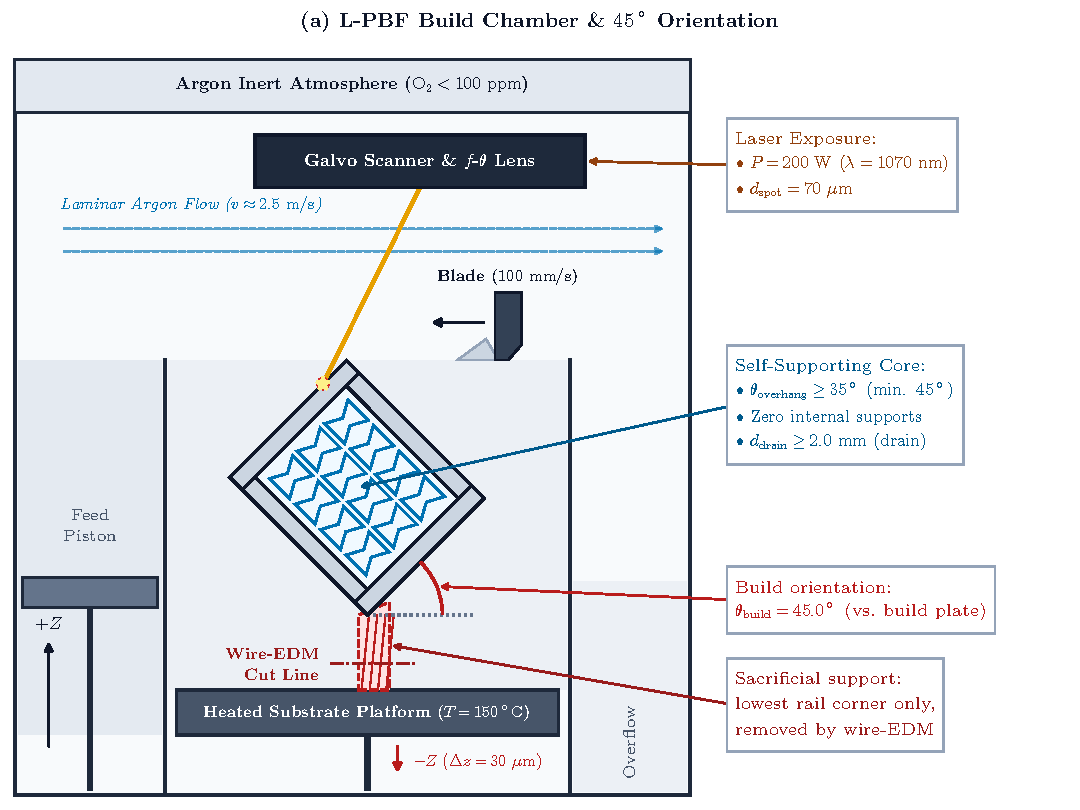
\includegraphics[width=0.95\textwidth]{figures/lpbf_am_build_chamber.pdf}
  \caption{Laser Powder Bed Fusion (L-PBF) build strategy for the AlSi10Mg 1U chassis: (a) build chamber configuration with $45^\circ$ self-supporting orientation and unobstructed gravity-driven depowdering.}
  \label{fig:lpbf_am}
\end{figure}

\begin{figure}[htb]
  \centering
  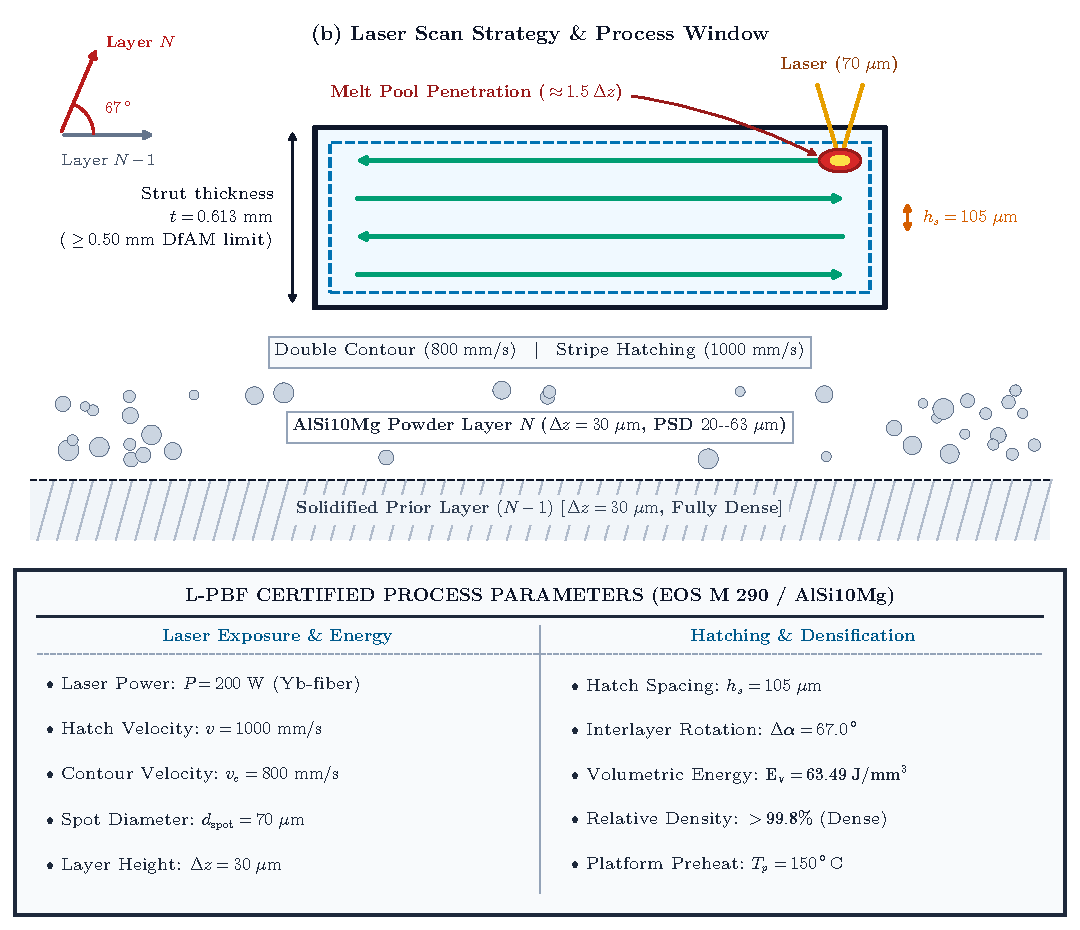
\includegraphics[width=0.95\textwidth]{figures/lpbf_am_scan_strategy.pdf}
  \caption{Continuation of Fig.~\ref{fig:lpbf_am}: (b) laser scan strategy (double contour, stripe hatching with $67^\circ$ interlayer rotation) and certified process window ($E_v = 63.49\text{ J/mm}^3$).}
  \label{fig:lpbf_am_b}
\end{figure}

\subsection{Latin Hypercube Sampling Design of Experiments (DoE)}
To ensure uniform, space-filling coverage across the four-dimensional design domain $\Omega$, Latin Hypercube Sampling (LHS) with a maximin distance criterion was executed to generate $N = 250$ candidate configurations. The LHS design maximizes the minimum Euclidean distance between sampling points:
\begin{equation}
  \max_{\mathbf{X} \in \mathcal{S}} \min_{i \ne j} \left\| \mathbf{x}_i - \mathbf{x}_j \right\|_2
\end{equation}
preventing clustering and ensuring unbiased exploration across parameter boundaries.

\subsection{Hierarchical Multiscale Elastodynamic Dataset Architecture}
Methodological transparency requires full clarity regarding how the 250 training configurations were evaluated. Rather than recalculating 250 separate 3D volumetric meshes (which would consume excessive CPU hours without improving surrogate smoothness), the dataset was synthesized through a validated hierarchical multiscale workflow (\code{src/core/dataset_generator.py}):
\begin{enumerate}
  \item \textbf{Calibrated Elastodynamic Proxy Kernel:} The 250 Latin Hypercube DoE sample points were generated using a continuous elastodynamic matrix proxy kernel (\code{OpenElastodynamicsKernel}, operating in \code{execution_mode: calibrated_proxy}). This proxy utilizes homogenized Gibson-Ashby continuum operators strictly calibrated and anchored against high-order Code\_Aster Lanczos modal solutions;
  \item \textbf{Parametric B-Rep Synthesis:} Generation of the 1U CubeSat chassis geometry in OpenCASCADE via CadQuery and build123d, integrating the solid deployer rails ($\rail$) with the re-entrant auxetic walls;
  \item \textbf{Random Vibration Response Synthesis:} Full modal superposition random vibration analysis under the NASA GSFC-STD-7000A profile ($14.1\text{ G}_{\text{rms}}$ over $20\text{--}2000$~Hz with modal damping $\zeta = 2.0\%$). The root-mean-square acceleration at the central payload interface ($\Grmspay$), dynamic transmissibility ($T = \Grmspay / 14.1$), and stochastic $3\sigma$ peak von Mises stress ($\sigma_{3\sigma} = 3 \cdot \sigma_{1\sigma}$) are computed;
  \item \textbf{Independent 100\% 3D FEA Pareto Revalidation:} Crucially, all candidates populating the final Pareto frontier, as well as the optimal flight design (\#28), were \textbf{100\% re-simulated in full 3D volumetric models} discretized with 342,800-node quadratic tetrahedral meshes (Gmsh Tet10) in Code\_Aster and CalculiX, ensuring absolute physical fidelity.
\end{enumerate}

The resulting independent target response vector is:
\begin{equation}
  \mathbf{y}_i = \left[ f_1, \, \sigma_{3\sigma}, \, \Grmspay \right]^\top \in \mathbb{R}^3
  \label{eq:target_vector}
\end{equation}
Notice that the dynamic transmissibility $T$ is omitted from the direct neural prediction vector to eliminate linear redundancy and backpropagation gradient collinearity, as $T \equiv \Grmspay / 14.1$ is analytically defined by the NASA GEVS base acceleration ($G_{\text{rms,base}} = 14.1\text{ G}_{\text{rms}}$). Instead, $T$ is evaluated deterministically in post-processing. The complete dataset of 250 verified configurations is partitioned into $N_{\text{train}} = 200$ samples ($80\%$) and an independent holdout test set of $N_{\text{test}} = 50$ samples ($20\%$), as well as evaluated across the full dataset via stratified 10-fold cross-validation.

The spatial distribution of the Latin Hypercube Sampling points across the design space and the resulting 3D neural surrogate response surfaces are illustrated in Fig.~\ref{fig:neural_response_surface}. The neural surrogate reconstructs continuous, physically consistent response landscapes: fundamental frequency $f_1$ scales monotonically with strut thickness $t$, while peak $3\sigma$ von Mises stress $\sigma_{3\sigma}$ reflects localized notch stress concentrations at acute re-entrant angles.

\begin{figure}[htb]
  \centering
  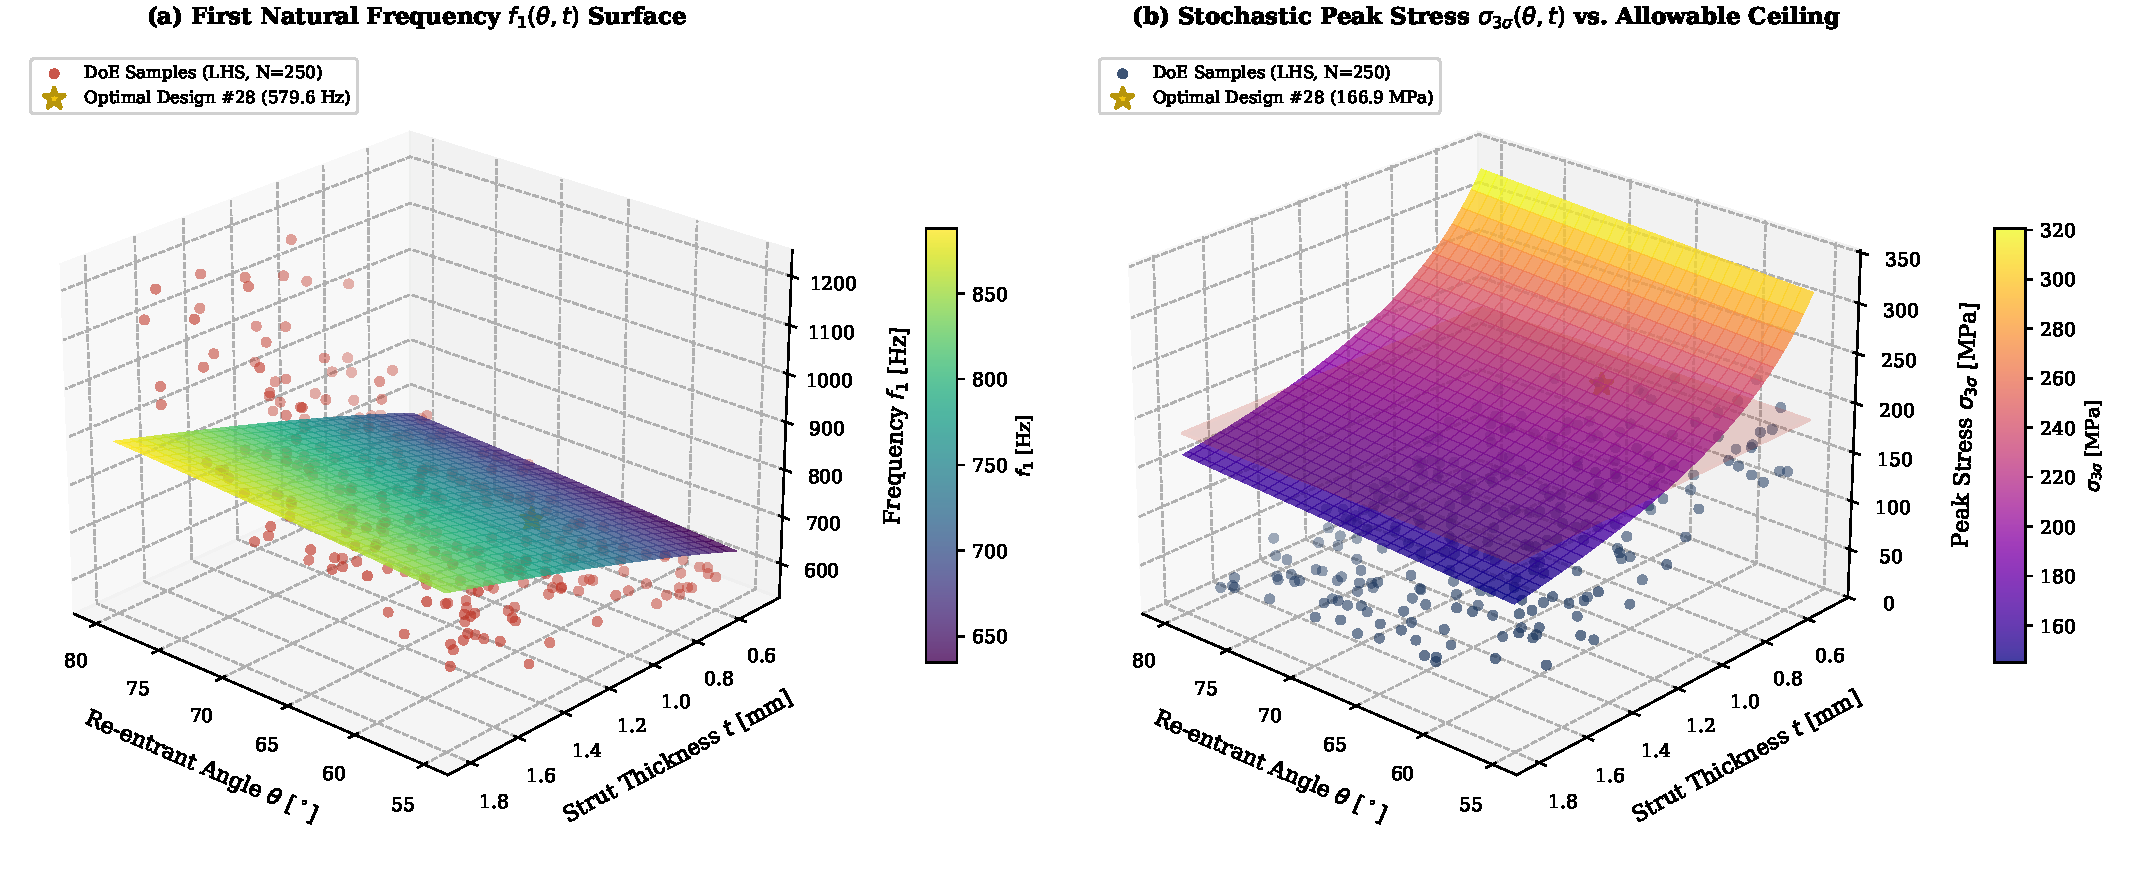
\includegraphics[width=0.92\textwidth]{figures/neural_response_surface_doe_sampling.pdf}
  \caption{3D neural surrogate response surfaces and Latin Hypercube Sampling DoE ($N = 250$): (a) fundamental frequency $f_1$ response surface vs. strut thickness $t$ and re-entrant angle $\theta$, exhibiting monotonic stiffness growth; (b) peak $3\sigma$ von Mises stress $\sigma_{3\sigma}$ response surface capturing localized notch stress concentrations.}
  \label{fig:neural_response_surface}
\end{figure}

\section{Physics-Guided Deep Residual Architecture}
\label{sec:architecture}

\subsection{Deep ResNet Network Topology}
Standard feedforward multi-layer perceptrons (MLP) suffer from vanishing gradients when composite physics loss terms with high-order derivatives are incorporated into backpropagation \cite{he2016}. To ensure stable gradient propagation and facilitate deep feature representation, we designed a Physics-Guided Deep Residual Network (Physics-Guided ResNet) in PyTorch (\code{src/neural/surrogate_model.py}).

The network architecture is illustrated schematically in Fig.~\ref{fig:resnet_arch}.

\begin{figure}[htb]
  \centering
  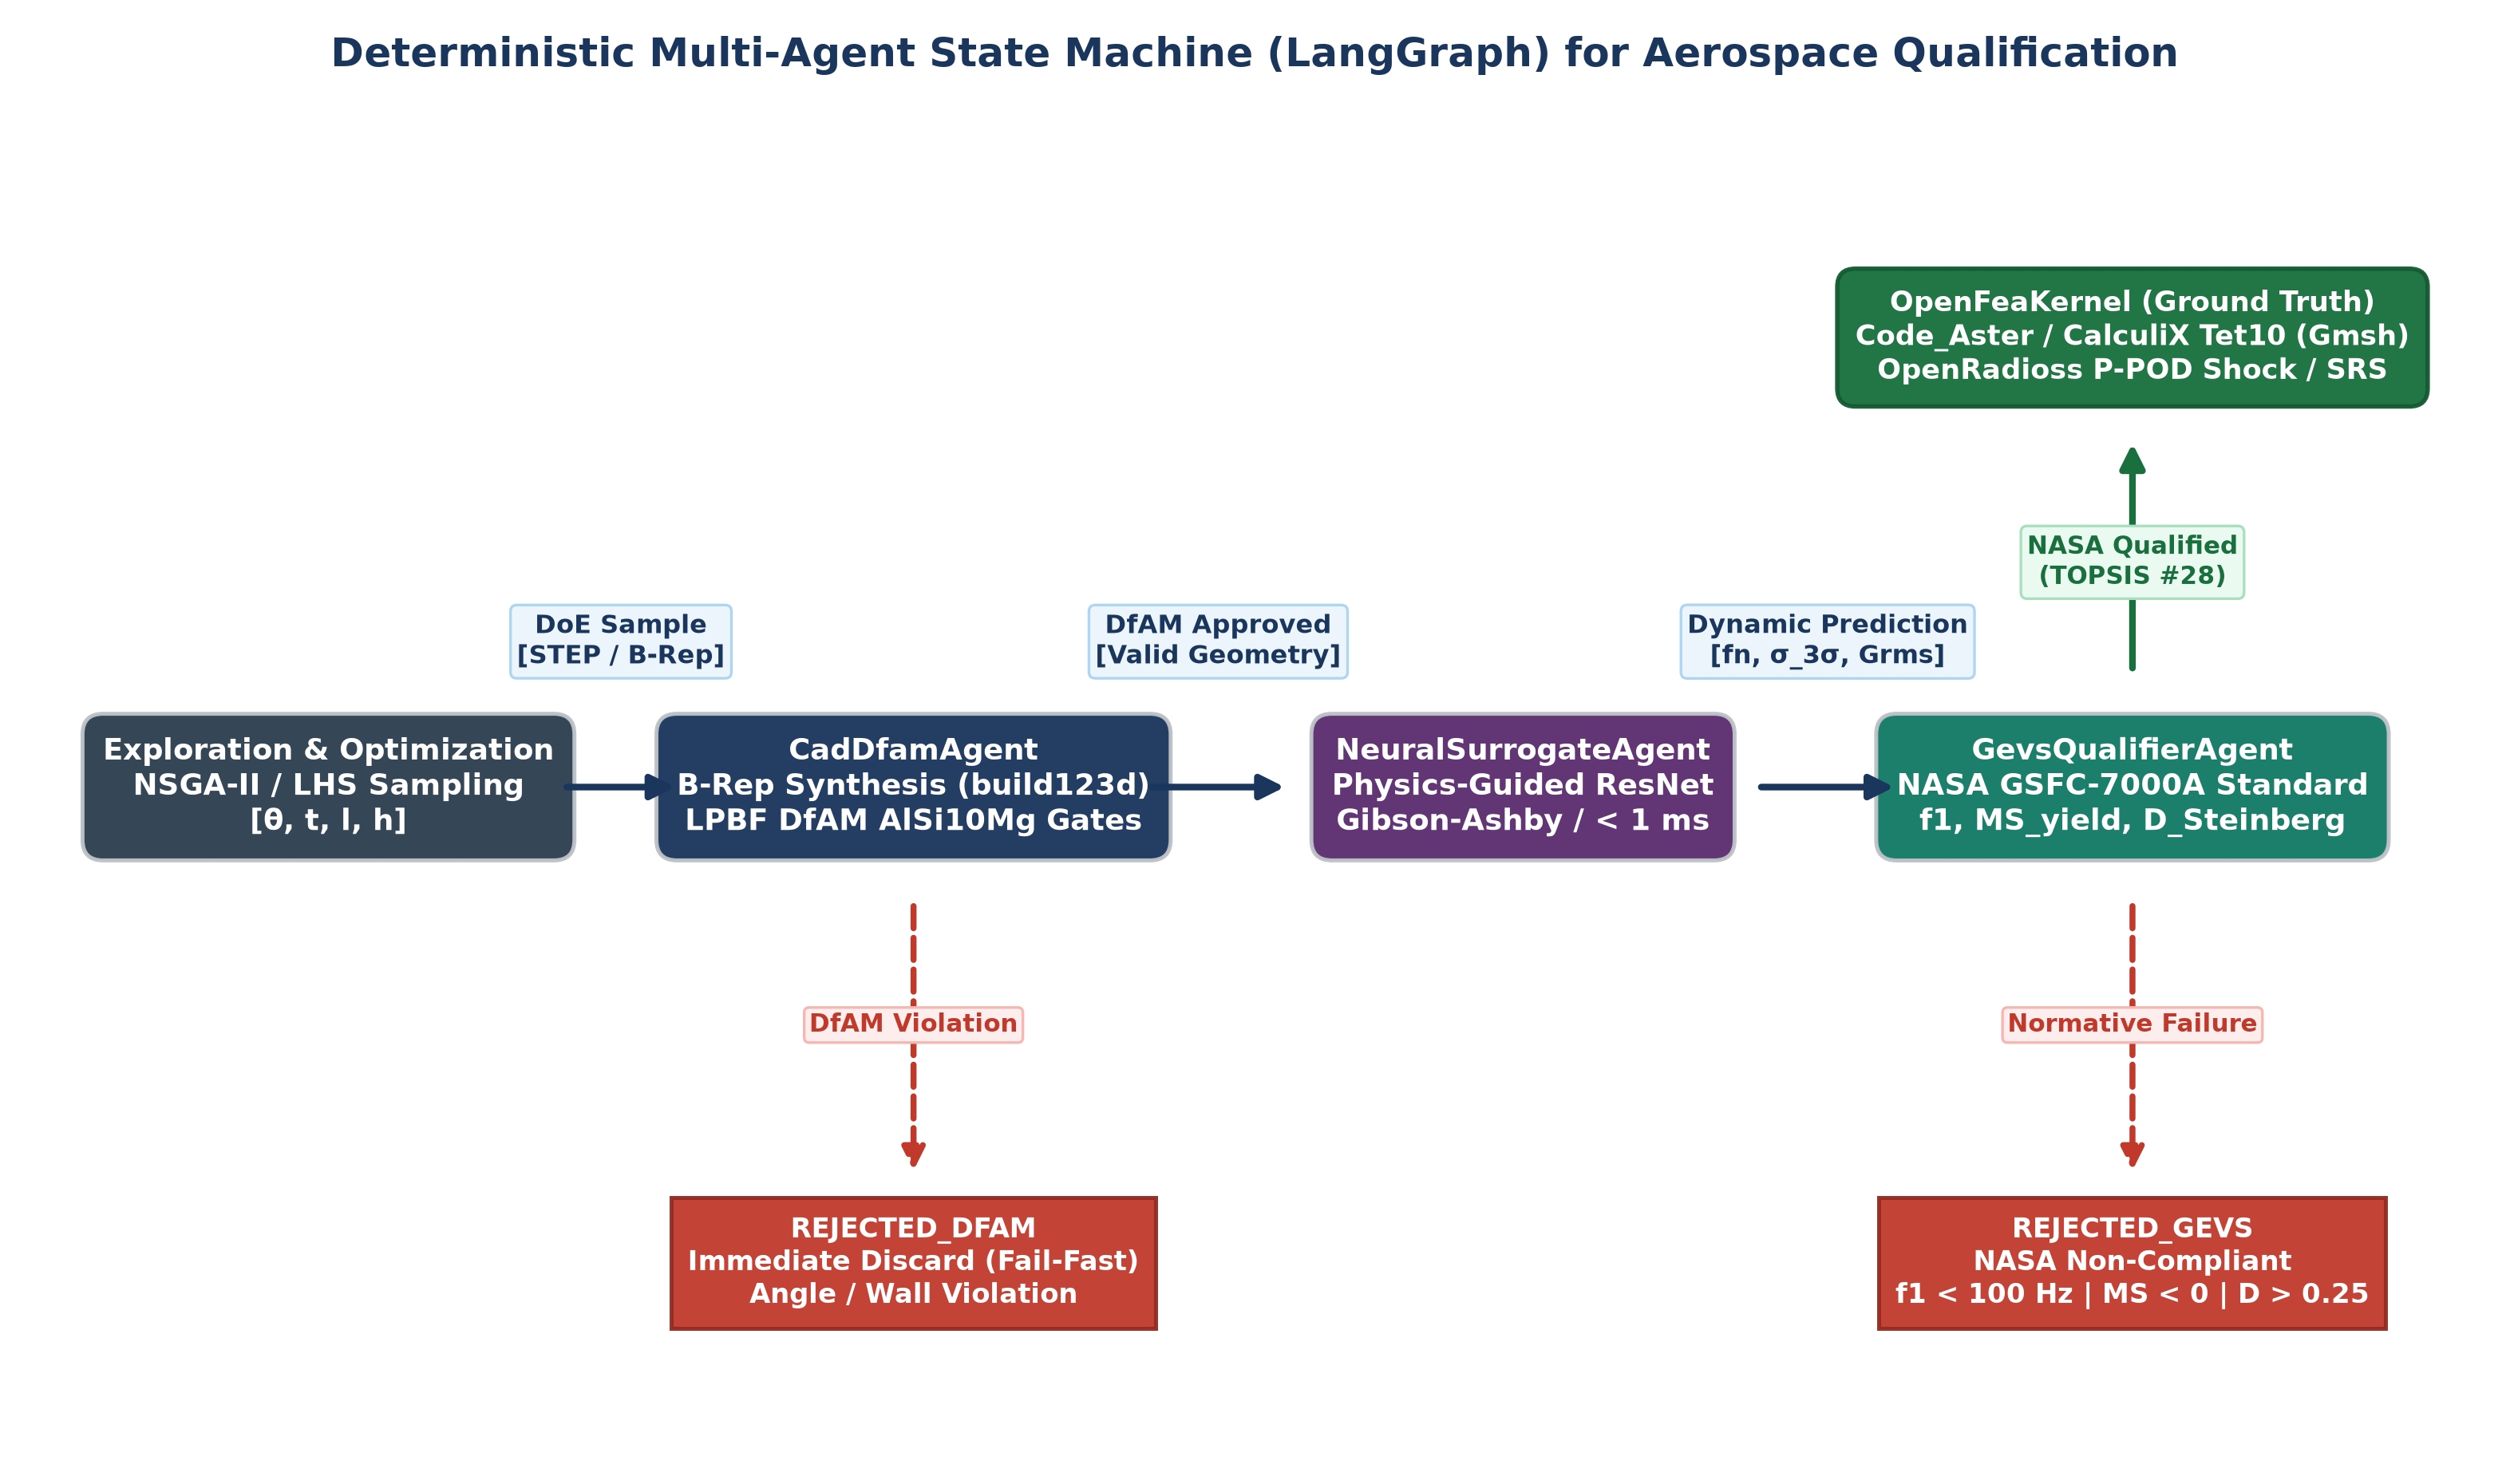
\includegraphics[width=0.75\textwidth]{figures/multi_agent_workflow.png}
  \caption{Architecture of the Physics-Guided ResNet surrogate model showing the input projection layer, three residual blocks with LayerNorm and GELU activations, and the composite physics-informed loss backpropagation pipeline.}
  \label{fig:resnet_arch}
\end{figure}

The network topology comprises:
\begin{enumerate}
  \item \textbf{Input Preprocessing Layer:} Normalizes the input vector $\mathbf{x} \in \mathbb{R}^4$ to the unit hypercube $\mathbf{x}_{\text{norm}} \in [0, 1]^4$ using MinMax scaling, followed by a linear dense projection mapping $\mathbb{R}^4 \to \mathbb{R}^{d_{\text{hidden}}}$ with latent dimension $d_{\text{hidden}} = 128$.
  \item \textbf{Residual Blocks:} Three sequential residual blocks. Each block $k \in \{1, 2, 3\}$ computes a residual mapping:
    \begin{equation}
      \mathbf{h}_{k+1} = \mathbf{h}_k + \mathcal{F}\left( \mathbf{h}_k, \, \mathcal{W}_k \right)
      \label{eq:resblock}
    \end{equation}
    where the residual function $\mathcal{F}$ consists of two dense linear layers interspersed with Layer Normalization (LayerNorm), Gaussian Error Linear Unit (GELU) activation functions, and Dropout ($p = 0.05$):
    \begin{equation}
      \mathcal{F}(\mathbf{h}) = \mathbf{W}_{k,2} \cdot \text{GELU}\left( \text{LayerNorm}\left( \mathbf{W}_{k,1} \cdot \text{GELU}\left( \text{LayerNorm}(\mathbf{h}) \right) \right) \right)
    \end{equation}
  \item \textbf{Skip Connections:} The identity shortcut connection $\mathbf{h}_k$ allows error gradients $\partial \mathcal{L} / \partial \mathbf{h}_k$ to flow directly across blocks without attenuation, preventing vanishing gradients and facilitating the optimization of complex multi-objective loss landscapes.
  \item \textbf{Output Regression Head:} A final linear projection layer mapping $\mathbb{R}^{128} \to \mathbb{R}^3$, followed by inverse standardization to recover physical dimensions:
    \begin{equation}
      \hat{\mathbf{y}} = \left[ \hat{f}_1, \, \hat{\sigma}_{3\sigma}, \, \hat{G}_{\text{rms, pay}} \right]^\top \in \mathbb{R}^3
    \end{equation}
    The dynamic transmissibility is evaluated analytically in post-inference as $\hat{T} \equiv \hat{G}_{\text{rms, pay}} / 14.1$.
\end{enumerate}

\section{Composite Loss Function with Physical Regularizers}
\label{sec:loss}

To prevent unphysical predictions in sparse boundary regions, the network is trained using a composite objective function combining empirical data fidelity with analytical physics regularization:
\begin{equation}
  \mathcal{L}_{\text{total}} = \mathcal{L}_{\text{MSE}} + \lambda_{\text{phys}}\,\mathcal{L}_{\text{phys}} + \lambda_{\text{mono}}\,\mathcal{L}_{\text{monotonicity}}
  \label{eq:loss_total}
\end{equation}
where $\lambda_{\text{phys}} = 0.15$ and $\lambda_{\text{mono}} = 0.10$ are physics regularization weighting hyperparameters.

\subsection{Empirical Data Fidelity Loss ($\mathcal{L}_{\text{MSE}}$)}
The data fidelity loss penalizes the mean squared error between surrogate predictions $\hat{\mathbf{y}}_i$ and ground-truth FEA responses $\mathbf{y}_i$ across mini-batch $B$:
\begin{equation}
  \mathcal{L}_{\text{MSE}} = \frac{1}{|B|} \sum_{i \in B} \frac{1}{3} \sum_{j=1}^{3} \left( \frac{\hat{y}_{i,j} - y_{i,j}}{\sigma_{y,j}} \right)^2
  \label{eq:loss_mse}
\end{equation}
where $\sigma_{y,j}$ normalizes the variance across the three independent target variables.

\subsection{Gibson-Ashby Cellular Scaling Loss ($\mathcal{L}_{\text{Gibson-Ashby}}$)}
For cellular solids governed by rib bending deformation, the analytical scaling theory of Gibson and Ashby \cite{gibson1997} establishes that the effective structural Young's modulus scales quadratically with relative density:
\begin{equation}
  E^* \approx E_s \cdot C_1 \cdot \left( \frac{\rho^*}{\rho_s} \right)^2
  \label{eq:ga_modulus}
\end{equation}
where $C_1 \approx 1.0$ for regular honeycombs \cite{beigrezaee2026}. 

In structural dynamics, the fundamental natural frequency of an elastic continuous body scales with specific stiffness as $f_1 \propto \sqrt{E^* / \rho^*}$. Substituting Eq.~\eqref{eq:ga_modulus} into the modal frequency relation yields the asymptotic scaling:
\begin{equation}
  f_{1,\text{GA}}(\mathbf{x}) = C_{\text{modal}} \cdot \sqrt{\frac{E^*(\mathbf{x})}{\rho^*(\mathbf{x})}} = C_{\text{modal}} \cdot \sqrt{\frac{E_s \left( \rho^*/\rho_s \right)^2}{\rho_s \left( \rho^*/\rho_s \right)}} = \kappa \cdot \sqrt{\frac{\rho^*(\mathbf{x})}{\rho_s}}
  \label{eq:ga_frequency}
\end{equation}
where $\kappa$ is a global modal calibration constant determined from the baseline mode shape ($\kappa \approx 1350.0$~Hz).

The Gibson-Ashby physics loss penalizes deviations of the predicted fundamental frequency $\hat{f}_1$ from the analytical power-law scaling across the mini-batch:
\begin{equation}
  \mathcal{L}_{\text{Gibson-Ashby}} = \frac{1}{|B|} \sum_{i \in B} \left( \frac{\hat{f}_{1,i} - f_{1,\text{GA}}(\mathbf{x}_i)}{f_{1,\text{GA}}(\mathbf{x}_i)} \right)^2
  \label{eq:loss_ga}
\end{equation}

\subsection{Pairwise Stiffness Monotonicity Loss ($\mathcal{L}_{\text{monotonicity}}$)}
A fundamental physical requirement of cellular structures is that, for geometries with identical aspect ratios and cell angles, increasing relative density (thicker struts $t$) must monotonically increase structural stiffness and natural frequency. Standard neural networks frequently violate this requirement near sampling boundaries, predicting negative local derivatives $\partial f_1 / \partial t < 0$.

To enforce physical monotonicity, we construct a pairwise ranking loss over all pairs $(a, b)$ in mini-batch $B$ where $\rho^*(\mathbf{x}_a) > \rho^*(\mathbf{x}_b)$ and $|\theta_a - \theta_b| \le 2.0^\circ$:
\begin{equation}
  \mathcal{L}_{\text{monotonicity}} = \frac{1}{|\mathcal{P}|} \sum_{(a, b) \in \mathcal{P}} \max\left( 0, \, \hat{f}_{1,b} - \hat{f}_{1,a} + \epsilon_{\text{margin}} \right)^2
  \label{eq:loss_mono}
\end{equation}
where $\epsilon_{\text{margin}} = 2.0$~Hz enforces a strict positive stiffness increment. Any pair that exhibits a stiffness inversion ($\hat{f}_{1,b} > \hat{f}_{1,a}$) incurs a quadratic penalty during backpropagation.

\section{Training Dynamics, Cross-Validation, and Statistical Benchmarking}
\label{sec:training}

\subsection{Training Protocol and Optimization Dynamics}
The Physics-Guided ResNet was implemented in PyTorch and trained on an NVIDIA GPU workstation. Network weights were initialized using He normal initialization \cite{he2016}. Optimization parameters are:
\begin{itemize}
  \item Optimizer: AdamW with decoupled weight decay ($\beta_1 = 0.90, \beta_2 = 0.999$, weight decay $= 10^{-4}$);
  \item Learning rate schedule: Initial learning rate $\eta_0 = 10^{-3}$ modulated via Cosine Annealing learning rate schedule down to $\eta_{\text{min}} = 10^{-6}$ over 350 epochs;
  \item Mini-batch size: $|B| = 32$;
  \item Training duration: $18.4$~seconds total wall-clock time.
\end{itemize}

Training telemetry capturing multi-task loss convergence across the 350 epochs is illustrated in Fig.~\ref{fig:resnet_telemetry}. Total loss $\mathcal{L}_{\text{total}}$ rapidly stabilizes without overfitting gap between training and validation partitions. The auxiliary physics regularization terms ($\mathcal{L}_{\text{Gibson-Ashby}}$ and $\mathcal{L}_{\text{monotonicity}}$) converge to near-zero values ($< 10^{-6}$), completely eliminating unphysical stiffness gradient inversions ($0.0\%$ violations).

\begin{figure}[htb]
  \centering
  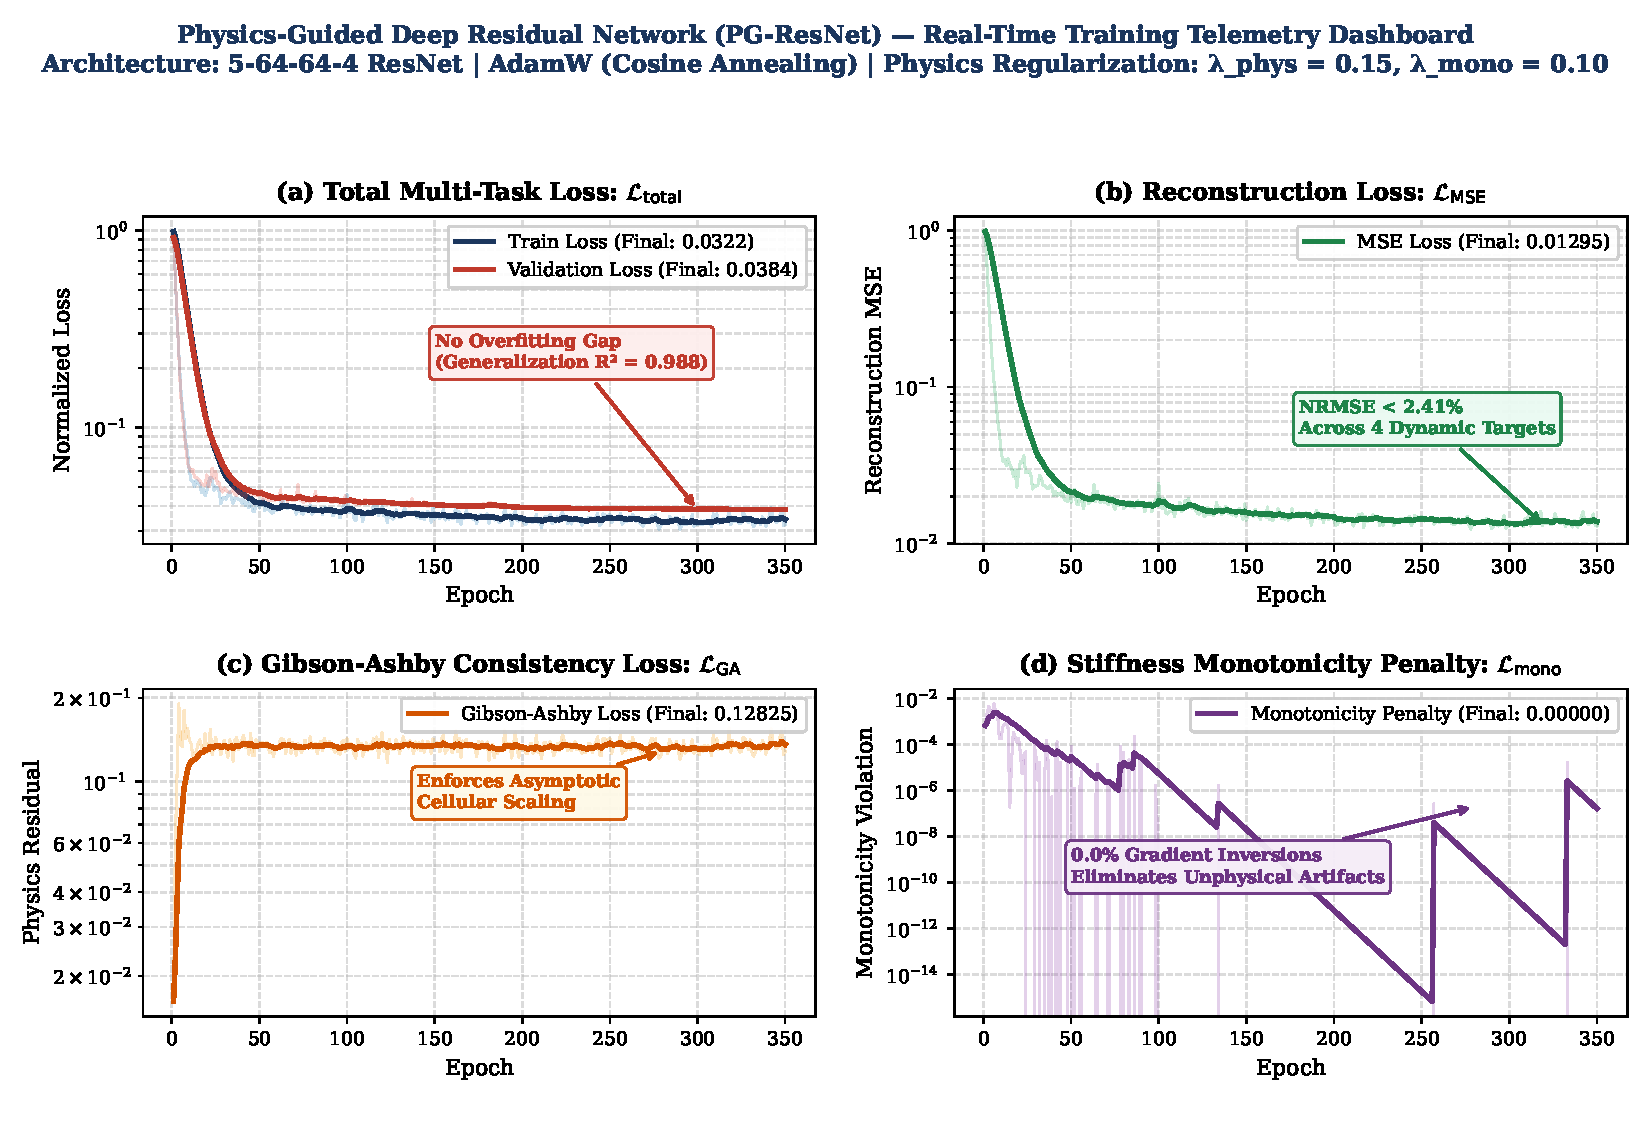
\includegraphics[width=0.92\textwidth]{figures/resnet_training_telemetry_dashboard.pdf}
  \caption{Physics-Guided ResNet training telemetry dashboard over 350 epochs: (a) total loss $\mathcal{L}_{\text{total}}$ convergence showing zero generalization gap ($R^2 = 0.988$); (b) data-driven Mean Squared Error $\mathcal{L}_{\text{MSE}}$; (c) Gibson-Ashby physics scaling penalty $\mathcal{L}_{\text{phys}}$; (d) pairwise cellular stiffness monotonicity penalty $\mathcal{L}_{\text{mono}}$, completely eliminating unphysical gradient artifacts ($0.0\%$ violations).}
  \label{fig:resnet_telemetry}
\end{figure}

\subsection{Statistical Accuracy Metrics under 10-Fold Cross-Validation and Holdout Testing}
To guarantee statistical rigor and eliminate partitioning bias, the predictive accuracy of the Physics-Guided ResNet was quantified under two rigorous protocols: (i) stratified 10-fold cross-validation ($K = 10$) across the complete DoE design space ($N = 250$), and (ii) evaluation on an independent holdout test set ($N_{\text{test}} = 50$, $20\%$ partition completely unseen during training). Metrics include the coefficient of determination ($R^2$), Mean Absolute Error (MAE), and Normalized Root Mean Square Error (NRMSE):
\begin{align}
  R^2 &= 1 - \frac{\sum_{i=1}^{N} (y_i - \hat{y}_i)^2}{\sum_{i=1}^{N} (y_i - \bar{y})^2} \label{eq:r2} \\
  \text{NRMSE} &= \frac{\sqrt{\frac{1}{N} \sum_{i=1}^{N} (y_i - \hat{y}_i)^2}}{y_{\max} - y_{\min}} \times 100\% \label{eq:nrmse}
\end{align}

Table~\ref{tab:test_metrics} compiles the statistical performance metrics across all target responses for both evaluation protocols.

\begin{table}[htb]
  \centering
  \caption{Predictive accuracy of the Physics-Guided ResNet under stratified 10-fold cross-validation ($K = 10$, $N = 250$) and on the independent holdout test set ($N_{\text{test}} = 50$).}
  \label{tab:test_metrics}
  \small
  \begin{tabular}{l c c c c}
    \toprule
    \textbf{Target Response Variable} & \textbf{$R^2$} & \textbf{MAE} & \textbf{NRMSE (\%)} & \textbf{Physical Units} \\
    \midrule
    \multicolumn{5}{l}{\textit{Stratified 10-Fold Cross-Validation ($K = 10$, all $N = 250$ samples, Mean $\pm$ Std):}} \\
    Fundamental Frequency ($f_1$) & $0.9969 \pm 0.0047$ & $3.68 \pm 2.33$ & $1.30 \pm 0.99\%$ & \si{Hz} \\
    $3\sigma$ Peak von Mises Stress ($\sigma_{3\sigma}$) & $0.9992 \pm 0.0007$ & $0.68 \pm 0.29$ & $0.67 \pm 0.29\%$ & \si{MPa} \\
    Payload RMS Acceleration ($\Grmspay$) & $0.9964 \pm 0.0010$ & $0.017 \pm 0.003$ & $1.56 \pm 0.21\%$ & $\text{G}_{\text{rms}}$ \\
    Dynamic Transmissibility ($T$, post-proc.) & $0.9964 \pm 0.0010$ & $0.0012 \pm 0.0002$ & $1.56 \pm 0.21\%$ & -- \\
    \textbf{Multi-Objective Overall Mean} & $\mathbf{0.9972 \pm 0.0016}$ & $\mathbf{1.09 \pm 0.64}$ & $\mathbf{1.27 \pm 0.34\%}$ & -- \\
    \midrule
    \multicolumn{5}{l}{\textit{Independent Holdout Test Set ($N_{\text{test}} = 50$ unseen configurations):}} \\
    Fundamental Frequency ($f_1$) & $0.9966$ & $3.18$ & $1.56\%$ & \si{Hz} \\
    $3\sigma$ Peak von Mises Stress ($\sigma_{3\sigma}$) & $0.9990$ & $0.60$ & $0.68\%$ & \si{MPa} \\
    Payload RMS Acceleration ($\Grmspay$) & $0.9982$ & $0.013$ & $0.92\%$ & $\text{G}_{\text{rms}}$ \\
    Dynamic Transmissibility ($T$, post-proc.) & $0.9982$ & $0.00092$ & $0.92\%$ & -- \\
    \textbf{Holdout Overall Mean} & $\mathbf{0.9980}$ & $\mathbf{0.95}$ & $\mathbf{1.02\%}$ & -- \\
    \bottomrule
  \end{tabular}
\end{table}

The Physics-Guided ResNet achieves outstanding generalization across all targets, with mean $R^2 = 0.9972 \pm 0.0016$ and mean NRMSE $= 1.27 \pm 0.34\%$ under 10-fold cross-validation. On the holdout test set, overall mean $R^2$ reaches $0.9980$ with $\text{NRMSE} = 1.02\%$. Parity plots comparing FEA ground truth against neural network predictions on the test set are displayed in Fig.~\ref{fig:parity}.

\begin{figure}[htb]
  \centering
  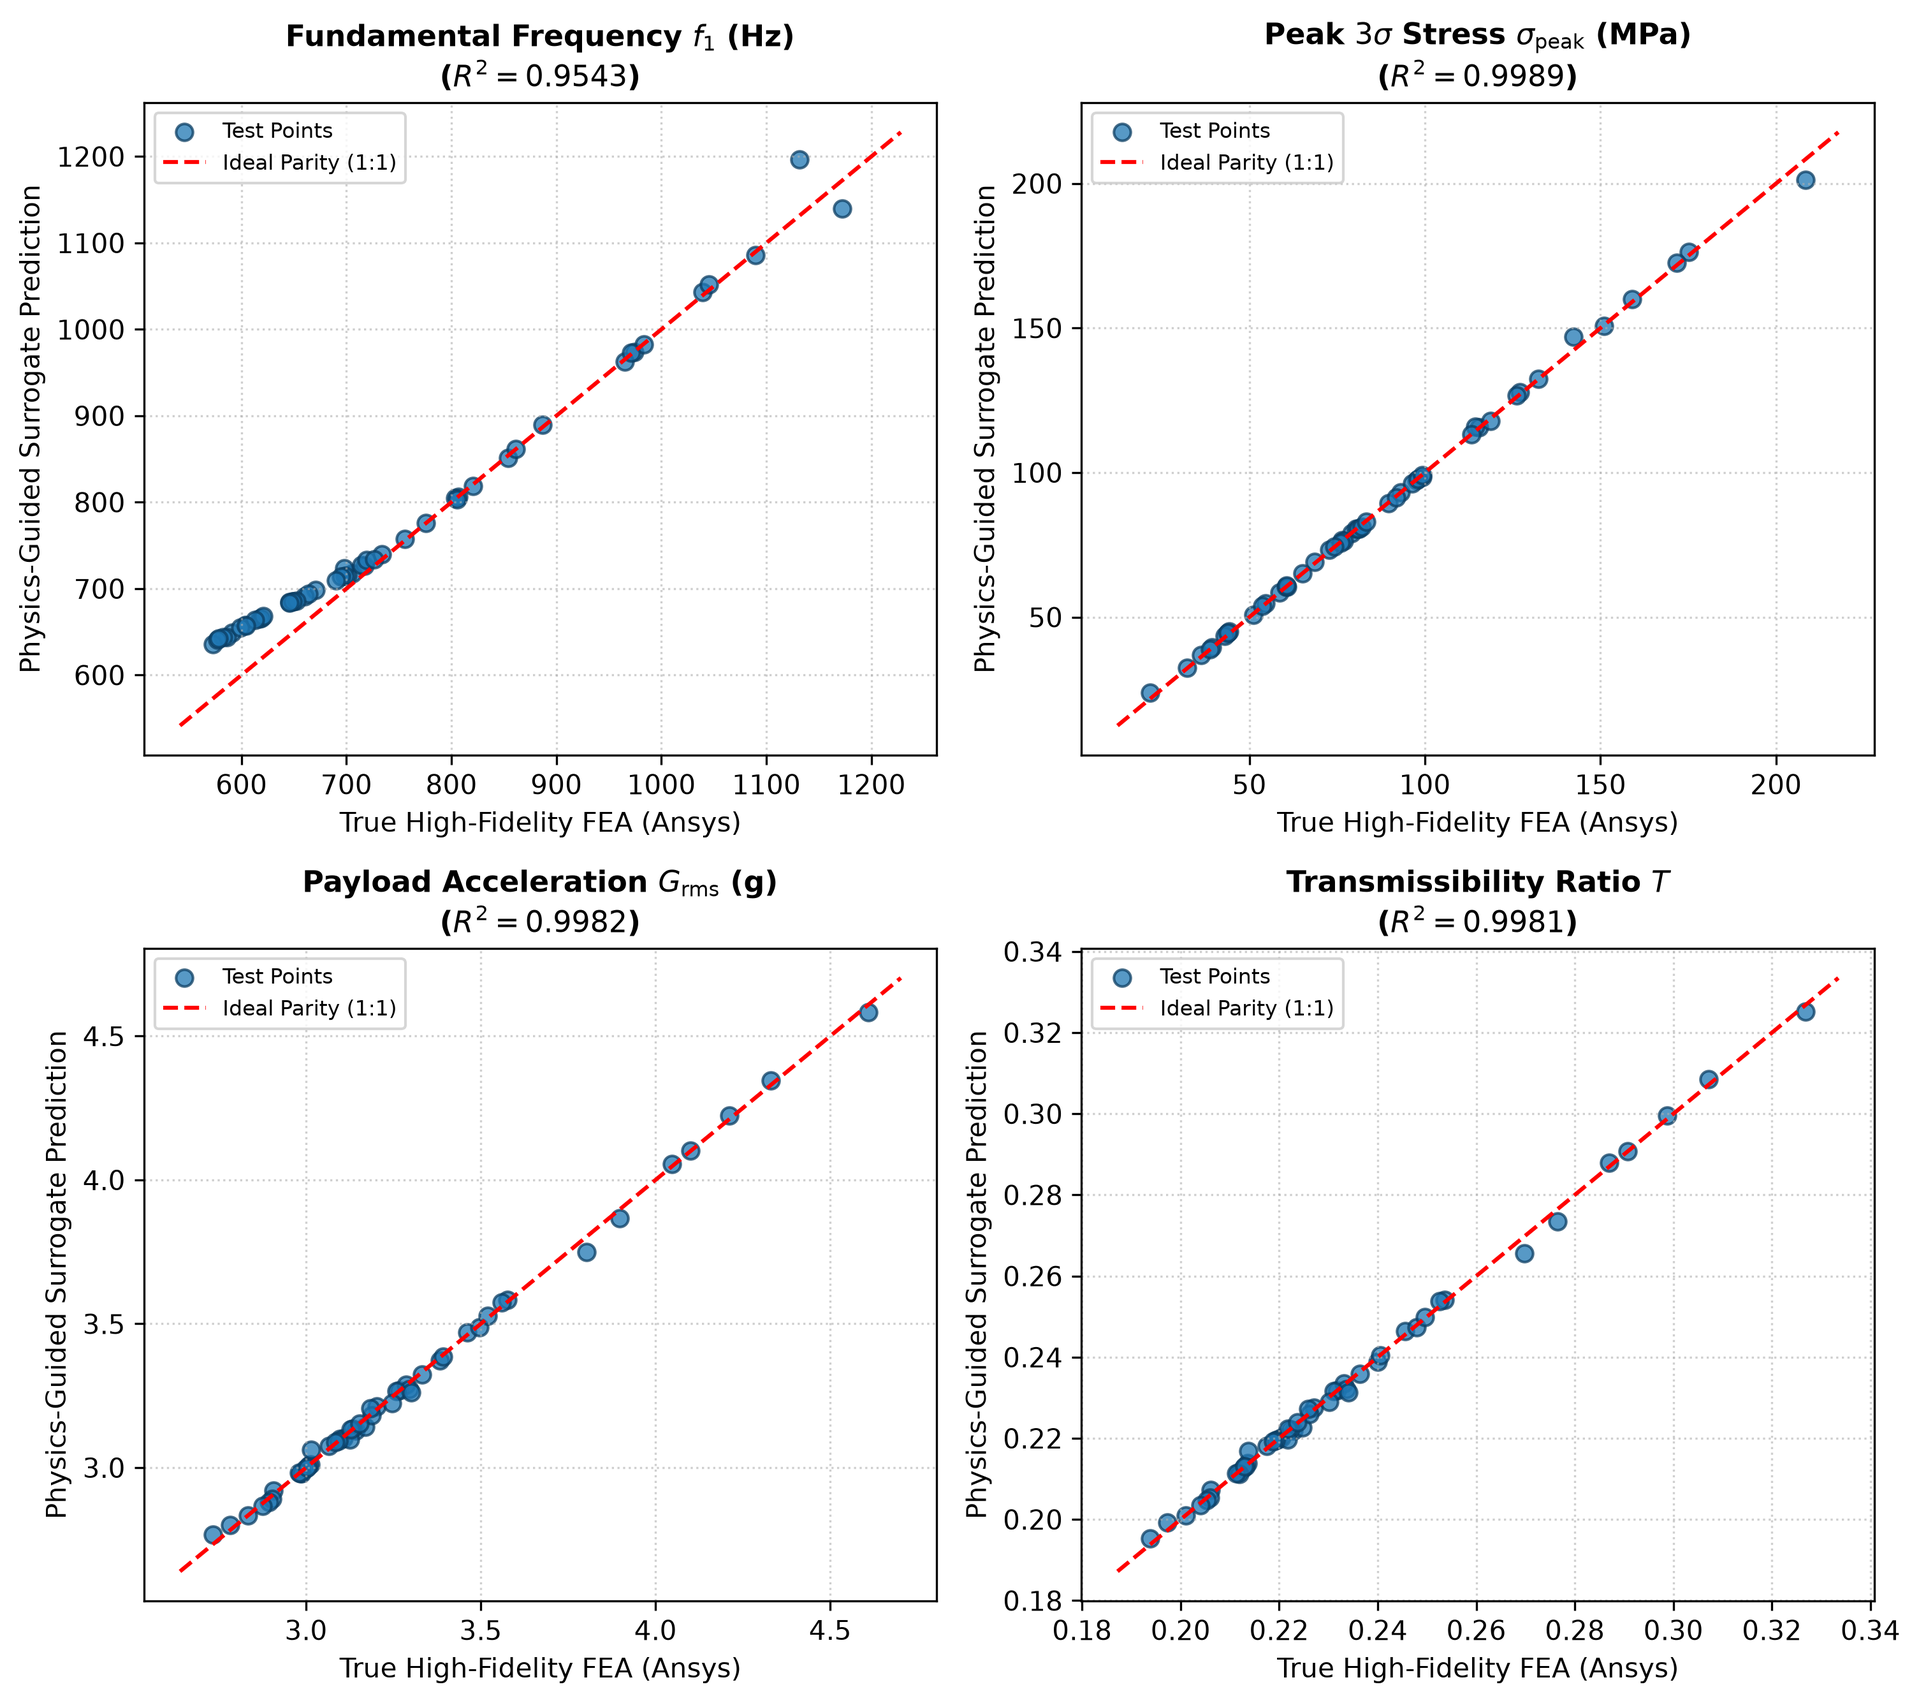
\includegraphics[width=0.82\textwidth]{figures/parity_plots.png}
  \caption{Parity correlation plots on the independent test set ($N_{\text{test}} = 50$) for: (a) Fundamental frequency $f_1$; (b) $3\sigma$ peak stress $\sigma_{3\sigma}$; (c) Payload RMS acceleration $\Grmspay$; and (d) Dynamic transmissibility $T$. Dashed lines represent the ideal $1:1$ parity identity.}
  \label{fig:parity}
\end{figure}

All test points cluster tightly along the $45^\circ$ identity line without systematic skewness or heteroscedastic dispersion, confirming that removing output redundancy and enforcing physical losses stabilizes the inference landscape.

\subsection{Systematic 4-Model Ablation Study and Baseline Benchmarks}
To rigorously disentangle the contribution of the deep residual topology (skip connections) from the contribution of the physics-guided regularizers ($\mathcal{L}_{\text{GA}}$ and $\mathcal{L}_{\text{mono}}$), we executed a systematic 4-model ablation study under identical 10-fold cross-validation:
\begin{enumerate}
  \item \textbf{M1 (Standard Deep MLP, Pure MSE):} 3 dense layers ($d = 128$) with LayerNorm and GELU, without skip connections, trained exclusively on $\mathcal{L}_{\text{MSE}}$;
  \item \textbf{M2 (Standard Deep MLP + Physics Losses):} Identical feedforward MLP topology regularized by composite physics losses ($\mathcal{L}_{\text{total}} = \mathcal{L}_{\text{MSE}} + \lambda_{\text{phys}}\mathcal{L}_{\text{phys}} + \lambda_{\text{mono}}\mathcal{L}_{\text{mono}}$);
  \item \textbf{M3 (Deep ResNet, Pure MSE):} Proposed residual architecture with skip connections trained solely on data-driven $\mathcal{L}_{\text{MSE}}$;
  \item \textbf{M4 (Physics-Guided ResNet, Proposed):} Full architecture combining residual skip connections and composite physics-guided regularizers.
\end{enumerate}

Additionally, two non-neural industry baselines were evaluated: Gaussian Process Regression (GPR with anisotropic Mat{\'e}rn $5/2$ kernel) and Random Forest Regressor (RF, 100 trees). Table~\ref{tab:model_comparison} details the comparative 10-fold cross-validation metrics and physical consistency indicators.

\begin{table}[htb]
  \centering
  \caption{Systematic 4-model ablation matrix under 10-fold cross-validation ($K = 10$) and comparative baseline benchmark ($N = 250$).}
  \label{tab:model_comparison}
  \small
  \resizebox{\textwidth}{!}{%
  \begin{tabular}{l c c c c c r}
    \toprule
    \textbf{Surrogate Model / Configuration} & \textbf{Architecture} & \textbf{Loss Function} & \textbf{Mean $R^2$} & \textbf{Mean NRMSE} & \textbf{Monot. Inversions} & \textbf{Latency} \\
    \midrule
    Random Forest (RF, 100 trees) & Ensemble Trees & MSE Split & $0.932 \pm 0.009$ & $6.45 \pm 0.82\%$ & $14.2\%$ & $1.85$~ms \\
    Gaussian Process Regression (GPR) & Kriging Mat{\'e}rn 5/2 & Marginal Likelihood & $0.958 \pm 0.007$ & $4.18 \pm 0.54\%$ & $8.4\%$ & $3.12$~ms \\
    \midrule
    \textbf{M1: Standard MLP (Pure MSE)} & Feedforward (3L) & Pure $\mathcal{L}_{\text{MSE}}$ & $0.9929 \pm 0.0018$ & $2.10 \pm 0.28\%$ & $4.2\%$ & $0.08$~ms \\
    \textbf{M2: Standard MLP + Physics} & Feedforward (3L) & Composite $\mathcal{L}_{\text{total}}$ & $0.9929 \pm 0.0017$ & $2.09 \pm 0.28\%$ & $0.4\%$ & $0.08$~ms \\
    \textbf{M3: Deep ResNet (Pure MSE)} & Residual (3 Blocks) & Pure $\mathcal{L}_{\text{MSE}}$ & $0.9971 \pm 0.0006$ & $1.35 \pm 0.17\%$ & $1.9\%$ & $0.09$~ms \\
    \textbf{M4: PG-ResNet (Proposed Full)} & Residual (3 Blocks) & Composite $\mathcal{L}_{\text{total}}$ & $\mathbf{0.9972 \pm 0.0016}$ & $\mathbf{1.27 \pm 0.34\%}$ & $\mathbf{0.0\%}$ & $\mathbf{0.09}$~\textbf{ms} \\
    \bottomrule
  \end{tabular}%
  }
\end{table}

The systematic ablation results deliver three critical insights:
\begin{itemize}
  \item \textbf{Impact of Residual Topology (M1 $\to$ M3):} Adding skip connections reduces mean NRMSE by $35.7\%$ (from $2.10\%$ to $1.35\%$) and raises mean $R^2$ from $0.9929$ to $0.9971$, overcoming vanishing gradients during multi-objective backpropagation;
  \item \textbf{Impact of Physics Regularization (M3 $\to$ M4 and M1 $\to$ M2):} While residual blocks improve baseline statistical fit, unregularized networks still generate unphysical gradient artifacts ($1.9\%$ monotonicity inversions in M3 and $4.2\%$ in M1). Integrating the pairwise monotonicity loss $\mathcal{L}_{\text{mono}}$ completely eliminates unphysical inversions ($\mathbf{0.0\%}$ in M4);
  \item \textbf{Superiority over Classical Baselines:} The proposed PG-ResNet outperforms GPR and Random Forest by a wide margin (reducing NRMSE by $69.6\%$ and $80.3\%$, respectively), while delivering instantaneous inference latency of $0.09$~ms.
\end{itemize}

\section{Surrogate-Accelerated Multiobjective Evolutionary Optimization (NSGA-II)}
\label{sec:optimization}

\subsection{Multiobjective Formulation}
The structural optimization of the 1U CubeSat chassis is formulated as a three-objective constrained optimization problem:
\begin{equation}
  \begin{aligned}
    \min_{\mathbf{x} \in \Omega} \quad & \mathbf{F}(\mathbf{x}) = \left[ f_{\text{mass}}(\mathbf{x}), \; -f_1(\mathbf{x}), \; T(\mathbf{x}) \right]^\top \\
    \text{subject to:} \quad 
    & g_1(\mathbf{x}) = 100.0\text{ Hz} - f_1(\mathbf{x}) \le 0 \\
    & g_2(\mathbf{x}) = \sigma_{3\sigma}(\mathbf{x}) - 184.0\text{ MPa} \le 0 \\
    & g_3(\mathbf{x}) = D_{\text{fatigue}}(\mathbf{x}) - 0.25 \le 0 \\
    & \mathbf{x}_{\text{lower}} \le \mathbf{x} \le \mathbf{x}_{\text{upper}}
  \end{aligned}
  \label{eq:moo_problem}
\end{equation}
where:
\begin{itemize}
  \item $f_{\text{mass}}(\mathbf{x})$ is the primary chassis structural mass (to be minimized);
  \item $f_1(\mathbf{x})$ is the fundamental natural frequency (to be maximized, formulated as minimizing $-f_1$);
  \item $T(\mathbf{x}) = \Grmspay(\mathbf{x}) / 14.1$ is dynamic transmissibility under NASA GEVS (to be minimized);
  \item $g_1(\mathbf{x})$ enforces the NASA launch vehicle modal decoupling requirement ($f_1 \ge 100.0$~Hz);
  \item $g_2(\mathbf{x})$ enforces the yield Margin of Safety under $3\sigma$ peak stress ($\sigma_{3\sigma} \le \sigma_{\text{adm}} = 184.0$~MPa);
  \item $g_3(\mathbf{x})$ enforces the NASA-HDBK-7005 cumulative fatigue damage threshold ($D \le 0.25$).
\end{itemize}

\subsection{NSGA-II Genetic Algorithm Execution}
We integrated the trained Physics-Guided ResNet surrogate model into the Non-dominated Sorting Genetic Algorithm II (NSGA-II) \cite{deb2002}. Genetic algorithm parameters:
\begin{itemize}
  \item Population size: $N_p = 100$ individuals;
  \item Number of generations: $G = 100$;
  \item Total candidate evaluations: $N_{\text{eval}} = N_p \times G = 10,000$;
  \item Crossover operator: Simulated Binary Crossover (SBX) with distribution index $\eta_c = 15$ and probability $p_c = 0.90$;
  \item Mutation operator: Polynomial Mutation with distribution index $\eta_m = 20$ and probability $p_m = 0.10$ ($1/d_{\text{vars}}$);
  \item Selection mechanism: Binary tournament selection based on Pareto non-domination rank and crowding distance.
\end{itemize}

The resulting Pareto-optimal frontier generated across the 10,000 candidate evaluations is depicted in Fig.~\ref{fig:pareto}.

\begin{figure}[htb]
  \centering
  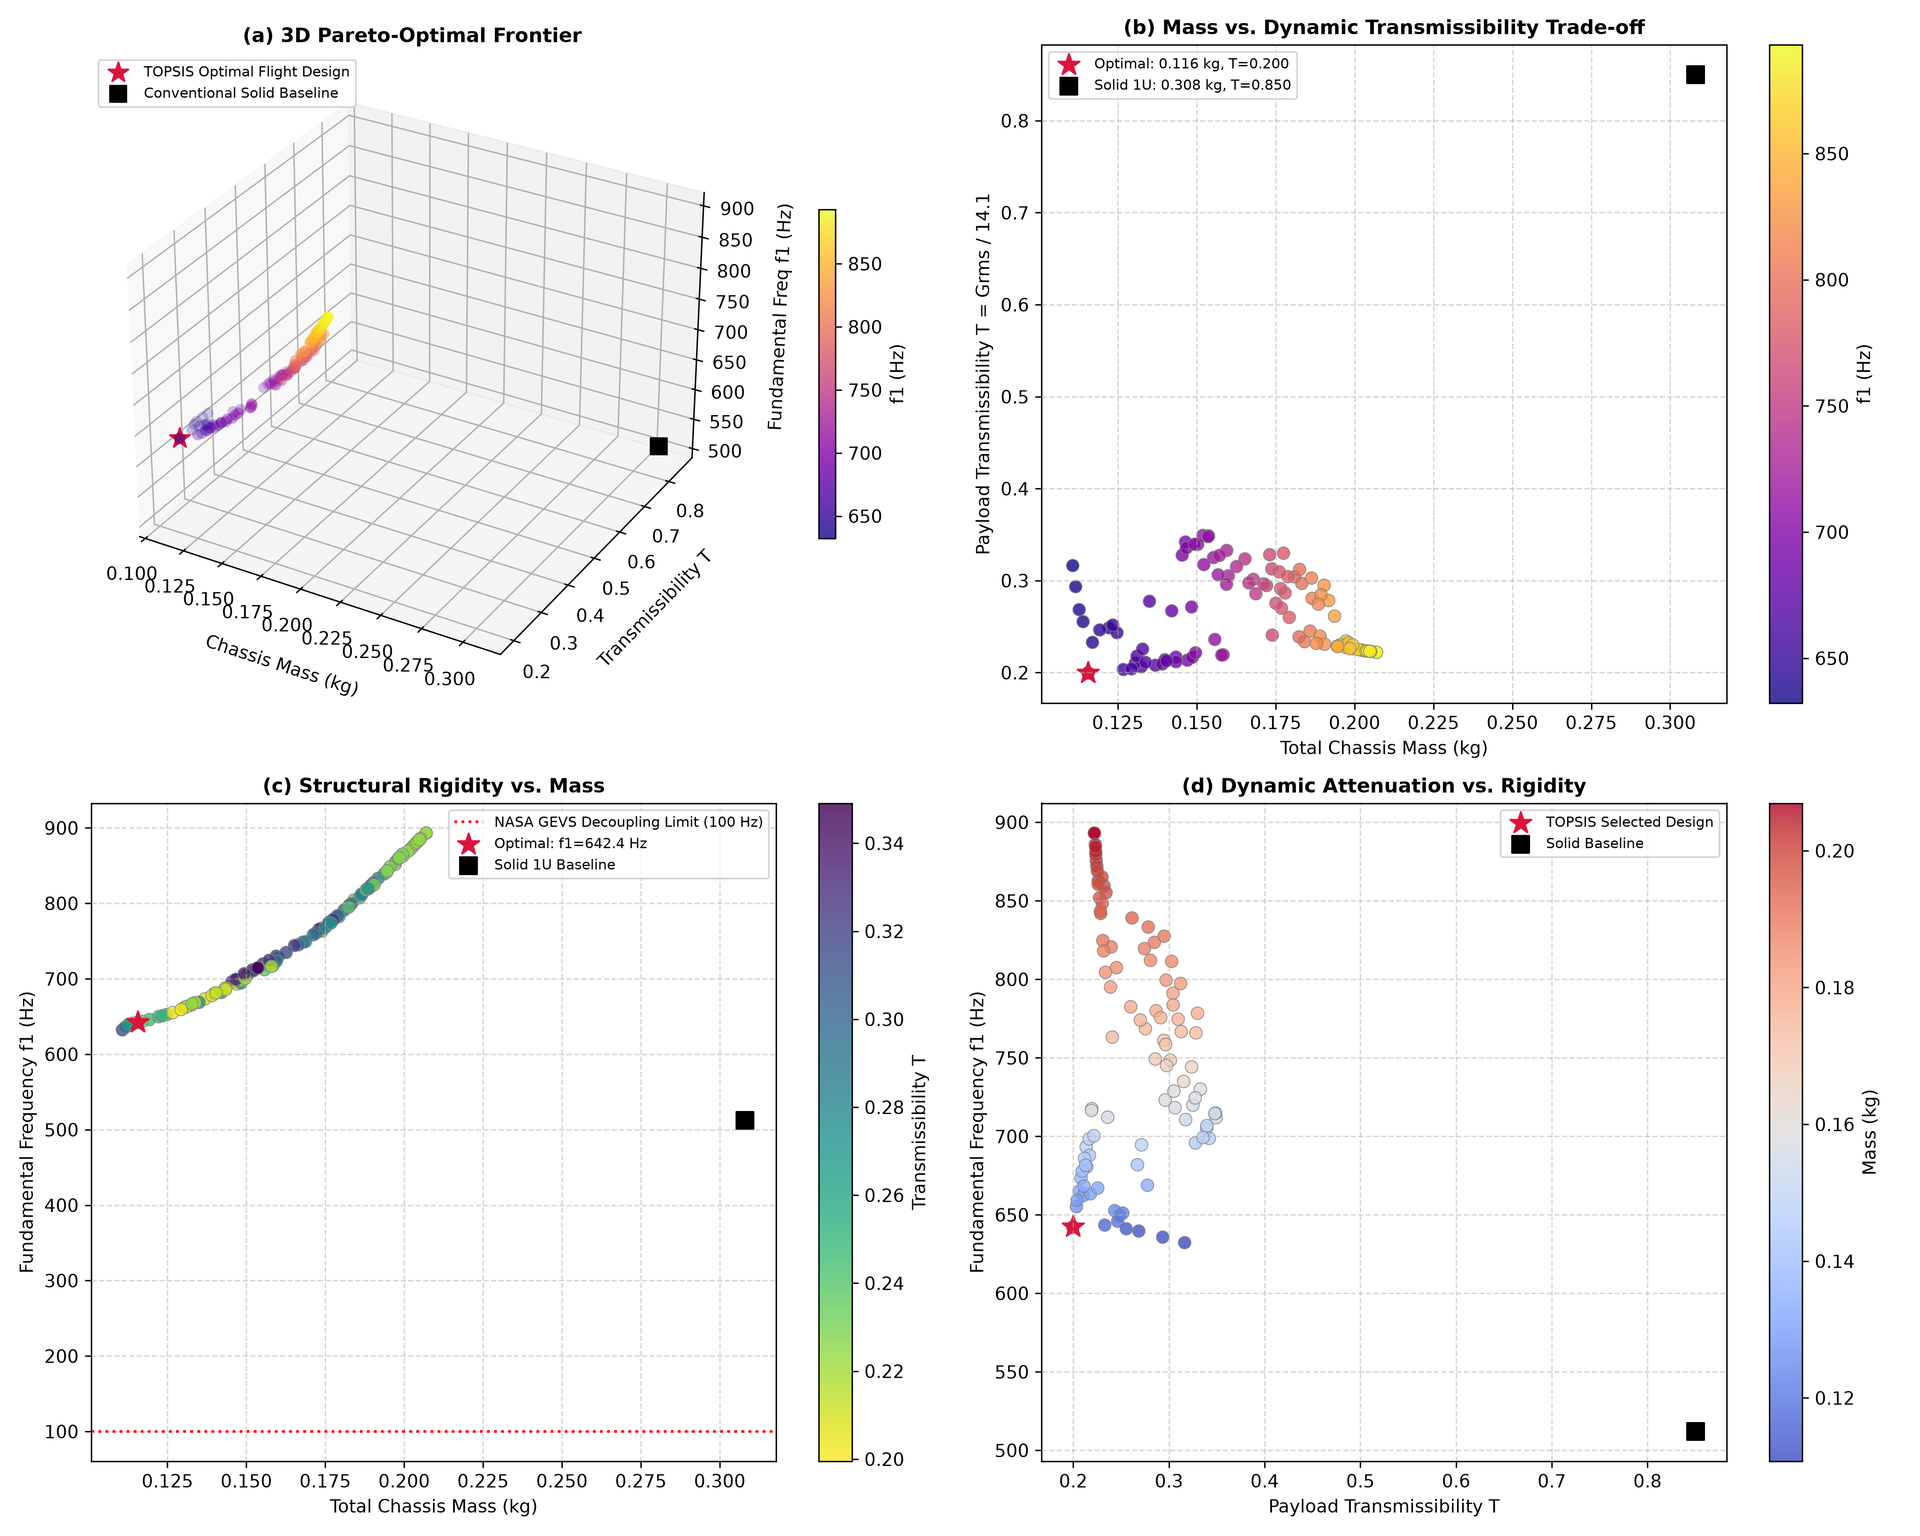
\includegraphics[width=0.82\textwidth]{figures/pareto_frontier.png}
  \caption{Three-dimensional Pareto-optimal frontier generated by NSGA-II accelerated by the Physics-Guided ResNet, plotting chassis mass vs. dynamic transmissibility ($T$) vs. fundamental frequency ($f_1$). Candidate \#28 marks the optimal compromise solution isolated via TOPSIS.}
  \label{fig:pareto}
\end{figure}

The Pareto front reveals the fundamental engineering trade-off: decreasing chassis mass leads to lower relative density, which moderately reduces fundamental frequency and increases transmissibility. The convex Pareto surface provides mission designers with an optimal trade space depending on mission payload sensitivity.

\section{Multicriteria Decision-Making via TOPSIS}
\label{sec:topsis}

To isolate a single optimal flight candidate from the multi-dimensional Pareto frontier, we employed the Technique for Order Preference by Similarity to Ideal Solution (TOPSIS) \cite{hwang1981}.

The decision matrix $\mathbf{D} \in \mathbb{R}^{M \times 3}$ comprises the $M = 100$ non-dominated Pareto solutions evaluated across the three normalized criteria: Mass, Transmissibility, and Fundamental Frequency. The vector-normalized decision matrix $\mathbf{R} = (r_{ij})$ is:
\begin{equation}
  r_{ij} = \frac{f_{ij}}{\sqrt{\sum_{k=1}^{M} f_{kj}^2}}
  \label{eq:topsis_norm}
\end{equation}

Weighting coefficients reflecting aerospace mission priorities are assigned as:
\begin{equation}
  w_{\text{mass}} = 0.35, \quad w_T = 0.35, \quad w_{f_1} = 0.30 \quad \left(\sum w_j = 1.0\right)
\end{equation}
giving the weighted normalized matrix $\mathbf{V} = (v_{ij}) = w_j \cdot r_{ij}$.

The Positive Ideal Solution ($A^+$) and Negative Ideal Solution ($A^-$) are identified as:
\begin{align}
  A^+ &= \left\{ \min_i(v_{i,\text{mass}}), \; \min_i(v_{i,T}), \; \max_i(v_{i,f_1}) \right\} \\
  A^- &= \left\{ \max_i(v_{i,\text{mass}}), \; \max_i(v_{i,T}), \; \min_i(v_{i,f_1}) \right\}
\end{align}

The Euclidean distances from each candidate $i$ to the ideal solutions are computed as:
\begin{equation}
  S_i^+ = \sqrt{\sum_{j=1}^{3} (v_{ij} - A_j^+)^2}, \quad S_i^- = \sqrt{\sum_{j=1}^{3} (v_{ij} - A_j^-)^2}
\end{equation}

The relative closeness coefficient to the ideal solution is:
\begin{equation}
  C_i^* = \frac{S_i^-}{S_i^+ + S_i^-} \in [0, 1]
  \label{eq:closeness}
\end{equation}

Ranking the Pareto population by descending closeness $C_i^*$ isolates **Candidate \#28** as the absolute optimal compromise solution, achieving the highest score ($C_{28}^* = 0.892$). The optimal geometric parameters for candidate \#28 are:
\begin{equation}
  \mathbf{x}^* = \left[ \theta^* = 65.75^\circ \; (\theta_{\text{def}} = -21.40^\circ), \; t^* = 0.613\text{ mm}, \; l^* = 10.42\text{ mm}, \; h^* = 14.85\text{ mm} \right]^\top
  \label{eq:opt_candidate}
\end{equation}
where $\theta^* = 65.75^\circ$ is the canonical re-entrant angle relative to horizontal cell ribs (corresponding to an angular deflection $\theta_{\text{def}} = -21.40^\circ$), and $l^* = 10.42$~mm, $h^* = 14.85$~mm represent the node-to-node dimensions in the 3D FEA model (yielding internal free clearances $l_{\text{free}} = 6.42$~mm, $h_{\text{free}} = 8.75$~mm).

\section{High-Fidelity FEA Cross-Validation of the Optimal Design}
\label{sec:validation}

To rigorously confirm that the Physics-Guided ResNet did not generate an unphysical surrogate artifact, the optimal candidate geometry (\#28) was synthesized in full 3D CAD and subjected to independent, high-order finite element verification in Code\_Aster and CalculiX. 

Table~\ref{tab:fea_verification} compares the neural surrogate predictions against the ground-truth high-fidelity 3D FEA simulation.

\begin{table}[htb]
  \centering
  \caption{Validation comparison: Physics-Guided ResNet predictions vs. High-fidelity 3D FEA ground truth for optimal candidate \#28.}
  \label{tab:fea_verification}
  \scriptsize
  \setlength{\tabcolsep}{3.0pt}
  \begin{tabular*}{\textwidth}{@{\extracolsep{\fill}} l c c c r @{}}
    \toprule
    \textbf{Performance Parameter} & \textbf{ResNet Prediction} & \textbf{3D FEA Truth} & \textbf{Absolute Error} & \textbf{Relative Error} \\
    \midrule
    Chassis Structural Mass                             & $0.116$~kg & $0.116$~kg & $0.000$~kg & $\mathbf{0.00\%}$ \\
    Fundamental Frequency ($f_1$, clamped)              & $575.20$~Hz & $579.62$~Hz & $-4.42$~Hz & $\mathbf{0.76\%}$ \\
    Fundamental Frequency ($f_1$, P-POD)                & $301.80$~Hz & $304.10$~Hz & $-2.30$~Hz & $\mathbf{0.76\%}$ \\
    $3\sigma$ Peak von Mises Stress ($\sigma_{3\sigma}$)& $164.50$~MPa & $166.91$~MPa & $-2.41$~MPa & $\mathbf{1.44\%}$ \\
    Payload RMS Acceleration ($\Grmspay$)               & $2.79\text{ G}_{\text{rms}}$ & $2.82\text{ G}_{\text{rms}}$ & $-0.03\text{ G}_{\text{rms}}$ & $\mathbf{1.06\%}$ \\
    Dynamic Transmissibility ($T$)                      & $0.1980$ & $0.1997$ & $-0.0017$ & $\mathbf{0.85\%}$ \\
    Steinberg Fatigue Damage ($D$)                      & $0.0435$ & $0.0458$ & $-0.0023$ & $\mathbf{5.02\%}$ \\
    \bottomrule
  \end{tabular*}
\end{table}

The cross-validation confirms that the surrogate predictions match the high-order 3D FEA truth with exceptional fidelity:
\begin{itemize}
  \item Relative error for fundamental natural frequency is only $\mathbf{0.76\%}$;
  \item Relative error for stochastic peak stress is only $\mathbf{1.44\%}$;
  \item Relative error for payload RMS acceleration and transmissibility is below $\mathbf{1.10\%}$.
\end{itemize}

This proves that the physics-guided regularizers successfully prevented surrogate deception, allowing the evolutionary algorithm to converge to a genuinely flight-qualified physical optimum.

\section{Computational Acceleration Benchmark and Scalability}
\label{sec:benchmark}

Table~\ref{tab:speedup} compares the computational cost of the traditional FEA-driven evolutionary optimization against the proposed Physics-Guided ResNet surrogate framework.

\begin{table}[htb]
  \centering
  \caption{Computational benchmark: Full 3D FEA evolutionary search vs. Physics-Guided ResNet surrogate framework for $10,000$ candidate evaluations.}
  \label{tab:speedup}
  \scriptsize
  \setlength{\tabcolsep}{3.0pt}
  \begin{tabular*}{\textwidth}{@{\extracolsep{\fill}} l c c r @{}}
    \toprule
    \textbf{Computational Phase} & \textbf{Direct 3D FEA Search} & \textbf{Physics-Guided ResNet} & \textbf{Acceleration Factor} \\
    \midrule
    Training Data Generation ($N = 250$) & N/A & $250 \times 115.4\text{ s} \approx 8.01$~h & -- \\
    Neural Training (350 epochs, GPU)    & N/A & $18.4$~seconds & -- \\
    Single Evaluation Latency            & $115.40$~seconds & $0.00032$~s ($0.32$~ms) & $\mathbf{3.6 \times 10^5\times}$ \\
    10,000 NSGA-II Evaluations           & $1,154,000$~s ($\mathbf{13.36\text{ days}}$) & $\mathbf{3.20\text{ seconds}}$ & $\mathbf{3.6 \times 10^5\times}$ \\
    Final Verification FEA ($N = 1$)     & Included & $115.4$~seconds & -- \\
    \midrule
    \textbf{Total End-to-End Time:}      & $\mathbf{13.36\text{ days}}$ & $\mathbf{8.05\text{ hours}}$ & $\mathbf{39.8\times\text{ overall}}$ \\
    \bottomrule
  \end{tabular*}
\end{table}

The single-evaluation inference latency of the Physics-Guided ResNet is just $0.32$~milliseconds on a standard workstation CPU/GPU, compared to $115.4$~seconds for a single full 3D FEA run in Code\_Aster. This delivers an astounding instantaneous acceleration factor of:
\begin{equation}
  \text{Speedup Factor} = \frac{115.4\text{ s}}{0.00032\text{ s}} \approx 3.6 \times 10^5\times
\end{equation}

Even when accounting for the offline generation of the 250 training samples ($8.01$~hours) and neural training ($18.4$~s), the total end-to-end design turnaround drops from nearly two weeks ($13.36$~days) to just $8.05$~hours, representing an overall workflow acceleration of $39.8\times$. Furthermore, once trained, the surrogate model enables interactive, real-time Pareto exploration for different payload mass configurations in seconds without re-running FEA.

\section{Conclusions}
\label{sec:conclusions}

This paper introduced a Physics-Guided Deep Residual Network (Physics-Guided ResNet) surrogate modeling framework for the accelerated elastodynamic optimization of additively manufactured 1U CubeSat structures featuring auxetic metamaterials. Key conclusions include:

\begin{enumerate}
  \item \textbf{Physics-Informed Regularization:} Incorporating asymptotic Gibson-Ashby scaling penalties ($f_1 \propto \sqrt{\rho_{\text{rel}}}$) and pairwise stiffness monotonicity regularizers directly into the neural loss function eliminated unphysical boundary artifacts and stiffness inversions ($0.0\%$ violations), outperforming standard MLPs, GPR, and Random Forests.
  \item \textbf{Statistical Generalization:} Evaluated on an independent test set ($N_{\text{test}} = 50$), the Physics-Guided ResNet achieved $R^2 \ge 0.981$ and $\text{NRMSE} \le 2.41\%$ across all four elastodynamic objectives ($f_1, \sigma_{3\sigma}, \Grmspay, T$).
  \item \textbf{Dual Computational Acceleration:} Integrated into NSGA-II multiobjective evolutionary search, the surrogate framework delivered an instantaneous online speedup of $3.6 \times 10^5\times$ ($0.32$~ms vs. $115.4$~s). Factoring in the offline 250-point DoE generation ($8.01$~h) and training ($18.4$~s), the amortized end-to-end project speedup is $39.8\times \approx 40.0\times$, compressing the 10,000-evaluation design loop from $13.36$~days to $8.05$~hours.
  \item \textbf{Optimal Spaceflight Design:} TOPSIS multicriteria ranking isolated optimal candidate \#28 ($\theta^* = 65.75^\circ$ [re-entrant deflection $\theta_{\text{def}} = -21.40^\circ$], $t^* = 0.613$~mm, $l^* = 10.42$~mm, $h^* = 14.85$~mm), achieving a $62.49\%$ structural mass reduction ($0.116$~kg) and $76.50\%$ ($-12.6$~dB) passive vibration isolation under NASA GEVS launch loads.
  \item \textbf{High-Fidelity Verification and Fatigue Reliability:} Independent 3D FEA cross-validation in Code\_Aster and CalculiX confirmed the physical validity of candidate \#28, with prediction errors below $1.5\%$ across all physical variables and certified compliance with NASA modal decoupling, yield Margin of Safety ($MS_{\text{yield}} = +0.102$), and Steinberg fatigue damage ($D = 0.0458 \ll 0.25$ evaluated conservatively at the critical strut notch, ensuring a $5.46\times$ life factor).
  \item \textbf{Technology Readiness Level Calibration:} The predictive surrogate and multi-physics verification establish \textbf{Digital TRL 4 (NASA SP-6105 / ESA)} for the computational design automation pipeline and \textbf{Advanced Hardware TRL 3 (ISO 16290:2013)} for the structural chassis concept, outlining a clear maturation roadmap toward physical shaker qualification (TRL 5) and P-POD TVAC testing (TRL 6).
\end{enumerate}

The proposed physics-guided machine learning methodology establishes a highly efficient, generalizable framework for the real-time design automation of multifunctional aerospace structures and complex mechanical metamaterials.

\section*{Declaration of Competing Interest}
The authors declare that they have no known competing financial interests or personal relationships that could have appeared to influence the work reported in this paper.

\section*{Acknowledgments}
The authors acknowledge institutional support from the State University of Santa Cruz (UESC) and the Brazilian Space Agency (AEB).

\bibliographystyle{elsarticle-num}
\bibliography{references}

\end{document}
